% =====================================================================
% LINGSHU -- main.tex
% Build:  pdflatex main && bibtex main && pdflatex main && pdflatex main
%
% File ownership (parallel writing; do not renumber inputs):
%   sections/01-abstract.tex .... A0   (this file's author)
%   sections/02-intro.tex ....... A0
%   sections/03-related.tex ..... A0
%   sections/04-problem.tex ..... A0
%   sections/05-method.tex ...... A4
%   sections/06-experiments.tex . A4
%   sections/07-discussion.tex .. A0
%   sections/08-limitations.tex . A4
%   sections/09-conclusion.tex .. A0
%   sections/10-appendix.tex .... A4
%
% Figures 1--2 are inserted by the lead inside 05-method.tex (Fig. 1) and
% 06-experiments.tex (Fig. 2). Fig. 3 (chaos state transitions) is inserted by
% A4 in 06-experiments.tex and is generated by paper/figures/fig3_robustness.py
% from experiments/chaos-injection/out/fig3-inputs.json. No graphics are required
% to compile this file beyond the PDFs already present in paper/figures/.
% =====================================================================
\documentclass[10pt,twocolumn]{article}

\usepackage[letterpaper,margin=0.75in]{geometry}
\usepackage[T1]{fontenc}
\usepackage[utf8]{inputenc}
\usepackage{times}
\usepackage{amsmath}
\usepackage{amssymb}
\usepackage{booktabs}
\usepackage{graphicx}
\usepackage{microtype}
\usepackage[numbers,sort&compress]{natbib}
\usepackage[hidelinks]{hyperref}
\usepackage{url}

% 英文版默认用 pdflatex 编译；若某个英文小节引用了中文原句（Mem0 试点语料），
% 用 xelatex 编译时自动加载 CJK 字体，保证这些字形不缺失。
\ifdefined\XeTeXversion
  \usepackage{xeCJK}
  \setCJKmainfont[Path=C:/Windows/Fonts/, Extension=.ttf]{simhei}
\fi

\setlength{\columnsep}{0.25in}
\setlength{\parskip}{0pt}
\frenchspacing

% Lightweight macros shared by all sections.
\newcommand{\system}{\textsc{LingShu}}
\newcommand{\host}{\textsc{Dsh}}
\newcommand{\eg}{e.g.,\ }
\newcommand{\ie}{i.e.,\ }
\newcommand{\wrt}{w.r.t.\ }

\title{\system: A Cybernetic Control Plane for Auditable\\
Cognition Plugins in Agent Hosts}

\author{\system{} Project Team\thanks{%
Preprint. Author list and affiliations will be finalized before submission.
Correspondence: the project's human owner (H0). This version reports the
state of the reference implementation as of October 2026.}}

\date{October 2026}

\begin{document}

\maketitle

\begin{abstract}
Persistent AI companions are where many users meet long-context agents: someone
raises a digital character over hundreds of turns, then it forgets its name or
catchphrase, and closing the session leaves it gone. The failure is less often
capability than the injection surface: memories are read as current facts,
stylistic signals soften refusals, persona constraints decay, and truncation can
push safety instructions out. We present \system{}, a deterministic and auditable
control plane that treats prompt assembly as a control surface. Six plugins share
one read-only constitutional boundary; a five-domain composer arbitrates among
them; and the control plane adds integral feedback with anti-windup, phase-shift
preemptive monitoring with persona anchors, requisite-variety reduction, and an
STPA-derived gate that structurally constrains what reaches the model at the
assembly boundary. Exactly one node is fail-closed---the STPA audit---so a
violation blocks injection instead of degrading it; every other component
degrades open and records why. The contract is machine-checkable: 892 Python
assertions across 14 files and 396 plugin-side assertions, with cross-copy
parameter consistency checked key by key. A chaos suite exercises each mechanism
in simulated and real hosts. We call the union the \emph{cyber-cognitive
envelope}; the name is ours, not a new mechanism.
\end{abstract}

\section{Introduction}\label{sec:intro}

Consider a persistent AI companion. A user raises a digital character over
hundreds of turns---practitioners sometimes call this ``cyber fish-keeping,''
slang rather than a research construct---and one day the character forgets its
own name or catchphrase; close the session, and it is gone. The motivation for
this work began as a simple wish: not wanting a virtual companion to die.

An interactive agent is not a single model call: before every call the host
assembles a prompt from memories, persona, goals, affect, and safety policy. In
short sessions this assembly is invisible; in long sessions it becomes the
dominant variable, because injected material grows while the budget does not.

Four failure modes follow, and they are the object of design throughout the
paper. \textbf{F1, memory overreach}: a stored memory is presented as a
statement of fact rather than as a reference to something the user once said.
\textbf{F2, refusal softening}: stylistic or affective signals are injected
into a turn that should be a refusal, and the refusal is weakened.
\textbf{F3, persona drift}: persona constraints stop influencing behaviour as
the context fills. \textbf{F4, budget capture}: truncation removes a
high-priority block while lower-priority stylistic blocks survive. Each is
observable at a specific point of the assembly pipeline, which makes them
tractable. We claim a control surface that is predictable, explainable and
rollbackable, and state its limits in Section~7.

\paragraph{Why structural, not only behavioural.} Alignment training shapes model
behaviour probabilistically: it lowers the rate of unsafe responses but does not
constrain what the host assembles around the model, nor certify after the fact
that a turn respected the policy. A structural layer complements it: decisions
are made in code at the assembly boundary before the model call, each decision is
recorded and replayable, and the one component whose failure is a safety failure
is fail-closed. The goal is not a better-behaved model but a prompt-assembly
surface whose behaviour can be constrained, observed and rolled back.

\paragraph{Positioning.} \system{} is not an attempt to make an agent more
human. Four senses of ``human-like'' are commonly conflated: capability
(remembering, forgetting, tracking goals), imperfection (misremembering, being
influenced by stale information), expression (tone, empathy, level of detail),
and self-claim (asserting feelings, needs, or subjective experience). We target
the first three and reject the fourth: it conflicts with the honesty property
the system should provide. The design goal is narrower: make
agent behaviour understandable, predictable, and trustworthy to the human in the
loop.

\paragraph{Five invariants.} Every component is constrained by five
invariants. \textbf{I1}: memory is a reference and never replaces the user's
current statement. \textbf{I2}: no full-history injection; context is a budget,
not a dump. \textbf{I3}: affect influences style only, never factual judgement.
\textbf{I4}: every inference is verbatim traceable, deniable, and rollbackable.
\textbf{I5}: plugins write only their own storage, and the memory plugin is the
single writer. A violation is a defect, not a trade-off.

\paragraph{Naming the control surface.} The mechanisms that police prompt
assembly---integral feedback, preemptive monitoring, dimensionality reduction,
and the pre-flight gate---are collectively what we call the
\emph{cyber-cognitive envelope}. The name is a framing device, not a new
mechanism: it denotes no separate code entity, each part is an ordinary module,
and no claim below depends on it.

\paragraph{Contributions.} Our contributions are structural and checkable; we
order them by how directly each one constrains the assembly boundary.

\begin{itemize}
\item \textbf{C1, a machine-checkable contract} (directly rerunnable). The
specification is not a document but assertions that fail loudly when a contract
breaks: 892 Python assertions across 14 test files, plus 396 plugin-side
assertions (188 host integration, 148 control-plane unit, 45 stress). Parameter
consistency between rules, engine, and plugin copies is itself machine-checked
(66 key comparisons).
\item \textbf{C2, one fail-closed locus} (pinned by regression tests). Exactly
one component is fail-closed---the STPA audit; everything else degrades open and
records why. Eight unsafe control actions are screened after assembly and before
the model call, and integral saturation is recorded as a downgrade rather than a
block. Mutation testing on the gate and memory-write paths kills
$42/42=100\%$ of non-equivalent mutants, with two equivalent mutants reported as
such.
\item \textbf{C3, structural defence at the assembly boundary} (measured, with a
stated boundary). Five domains are composed under a frozen order and eight
mutual-exclusion rules; what survives composition is screened by the gate. The
envelope therefore structurally constrains what reaches the model and fails
closed on violation, rather than asking the model to comply. Where its lexical
coverage ends is measured rather than assumed (Section~7).
\item \textbf{C4, an evaluation discipline and a documented port} (artefacts
exist and are machine-checked). Every parameter carries a provenance tag; the
instrument (metric definitions, replay set, guardrail thresholds) is frozen and
read-only for the learning loop; changes to it are rejected by an auditor. The
same control semantics exist twice, in a zero-dependency Python reference
implementation and a JavaScript host plugin, and the five known divergences are
listed rather than hidden.
\end{itemize}

\paragraph{Scope of the evidence.} The paper reports two kinds of evidence.
Contract feasibility: the specification executes and violation is observable.
Mechanism reachability: in the tested configuration each mechanism fires in a
real host session, with sample sizes stated. It also reports one negative result
that shaped the design: replacing exponential decay with a pure ACT-R base-level
activation drops \texttt{recall@3} on the frozen replay set from 1.000 to 0.556,
which is why the implemented model is a dual-channel maximum rather than a
replacement. Effect sizes on real traffic and the calibration of design-default
parameters are outside this paper's scope; Section~7 states what the current
evidence supports.

Section~\ref{sec:related} reviews related work, Section~\ref{sec:problem}
formalizes the problem, Sections~4--5 present mechanisms and evidence, and
Sections~6--8 discuss costs, limits, and conclusions.

\section{Related Work}\label{sec:related}

\paragraph{Long-term memory for agents.} Recent work treats agent memory as an
architecture rather than a vector store. ZenBrain proposes a seven-layer,
neuroscience-derived memory architecture with sleep-phase consolidation and
explicit ablations of each mechanism~\cite{zenbrain2026}. FSFM argues that
selective forgetting deserves first-class treatment and gives a taxonomy of
passive decay, active deletion, safety-triggered forgetting, and adaptive
reinforcement~\cite{fsfm2026}. A human-inspired architecture combines
sleep-phase consolidation, interference-based forgetting, and multi-cue
retrieval, reporting retention precision of 97.2\% at a 58\% store
reduction~\cite{himemory2026}. PersMem internalizes personality into a
dual-pathway memory pipeline so that memory processing becomes
personality-dependent~\cite{persmem2026}. Mem0 extracts, consolidates and
retrieves salient conversational facts at production scale, reporting large
latency and token savings over full-context prompting~\cite{mem0_2025}. These
systems optimize what is remembered and how well it is retrieved. Our concern is
different and orthogonal: what is \emph{allowed} to enter the prompt, under which
priority, and what happens when the budget cannot hold everything. We use Mem0 as
an external memory baseline for that question
(Section~\ref{sec:exp:baselines}).

\paragraph{Activation and decay.} Ranking memories over long horizons is usually
framed as a decay or activation problem. The ACT-R base-level activation folds
frequency and recency into a single logarithmic quantity, motivated by the
statistics of practice and need probability~\cite{anderson1991,anderson2007}.
We treat it as one of two channels rather than as a replacement for decay,
because an outright replacement degrades a frozen ranking baseline in our own
setting, as reported in Section~4. This is a concrete example of a general
point: borrowed mechanisms rarely transplant without a regression check against
the instrument that existed before the borrowing.

\paragraph{Affect and persona.} Sentipolis couples a continuous
Pleasure--Arousal--Dominance representation with dual-speed emotion dynamics
and emotion--memory coupling for social simulation~\cite{sentipolis2026}. Its
own report is instructive: gains are model-dependent, and emotion-awareness can
mildly reduce adherence to social norms. PAD itself dates back to environmental
psychology~\cite{mehrabian1974}. We adopt PAD as a representation and, unlike
simulation-oriented systems, confine affect to the style domain: an invariant
forbids affect from entering factual judgement, and the composer enforces the
separation structurally.

\paragraph{Safety engineering.} STPA analyses unsafe control actions in
safety-critical systems~\cite{leveson2011,leveson2018}. We adapt the notion of
an unsafe control action from its original, offline analytical setting to a
runtime gate: eight control actions are screened after composition and before
the model call, with a single fail-closed locus. The transfer is deliberate but
partial---STPA is a hazard-analysis method, whereas our gate is a predicate
evaluated on every turn---and we do not claim that our gate is a substitute for
a full STPA of the host.

\paragraph{Cybernetics and requisite variety.} Ashby's law of requisite variety
states that a regulator must command at least as much variety as the
disturbances it faces~\cite{ashby1956}; Beer's Viable System Model is one
influential reading of layered regulation~\cite{beer1972}. We borrow the
engineering idea that when a controller cannot represent a conflict, it should
shrink its own action space instead of acting anyway, and implement this as
dimensionality reduction over composition domains. We use VSM only as an
interpretive lens on an existing priority layering: it is borrowed, not
implemented, has no code locus, parameter, or dependency in our implementation,
and we do not claim System~1--5 machinery. Anti-windup for integral controllers
is standard control practice~\cite{astrom2006} and is adopted directly.

\paragraph{Evaluation and staged change.} Optimizing a single proxy invites
Goodhart's law~\cite{goodhart1975}, so our learning loop pairs every primary
metric with an adversarial counterpart, treats user corrections as the final
judge, and freezes the evaluation instrument itself. Change management follows
a conventional staged-rollout pattern (small share, guardrails, automatic
rollback), with the additional constraint that data insufficient to verify a
guardrail blocks release instead of skipping it.

\paragraph{Scope.} The mechanisms discussed above are the whole of the paper's
scope. Limits of that scope, including components that exist in the project but
are deliberately not claimed here, are stated in Section~7.

\section{Problem Formulation}\label{sec:problem}

\paragraph{Setting.} Let $H$ be an agent host and let turn $t$ have context
window $W_t$ and injection budget $B$. Before the model call, the host composes
a prompt from the user message and a set of injected blocks $D_t$, drawn from
five domains: \emph{safety} (whether to refuse), \emph{fact} (what to claim),
\emph{organization} (whether to offer options or narrate), \emph{style} (tone,
detail, address), and \emph{retrieval} (which retrieval strategy). Blocks have a
frozen assembly order, a frozen priority order inside each domain, and a
mutual-exclusion table across domains. Dynamic weights decide which block is
sacrificed when the budget is exceeded; they never decide which invariant may be
overridden.

\paragraph{Control actions.} A control plane acts on the composition through
five actions,
$U_t \in \{\text{\textsc{inject}}, \text{\textsc{reduce}},
\text{\textsc{anchor}}, \text{\textsc{trip}}, \text{\textsc{log}}\}$:
select blocks, shrink the represented domains, insert boundary anchors, block
the turn, and record a trace. Every action is a pure function of state that is
available before the model call.

\paragraph{Failure predicates.} The failures of Section~\ref{sec:intro} are
defined as predicates over the composition result, not over model output. Let
$\mathit{prefeed}_t$ be the preemptive-monitoring flag and $\mathit{blocks}_t$
the assembled block list; then
\begin{align}
F_1 &: \text{fact block asserts an unsourced memory statement},\\
F_2 &: \mathit{refuse}_t \wedge \text{a style block is present},\\
F_3 &: \mathit{prefeed}_t \wedge \text{no anchor marker in the prompt},\\
F_4 &: \text{the constitutional block is absent or not first}.
\end{align}
Each predicate is evaluated from the per-turn event without a model call, and
each maps to an unsafe control action in the gate (UCA-04, UCA-03, UCA-07,
UCA-05 respectively). Defining failure on the injection side rather than on the
answer is the design decision that makes the system auditable
deterministically: two runs with the same state and budget produce the same
verdict.

\paragraph{Evaluation instrument.} The instrument is a tuple
$(\mathcal{M}, \mathcal{R}, \mathcal{G})$: metric definitions $\mathcal{M}$
(recall@3 over expected identifiers, forbidden-identifier leakage, truncated
turns), a replay set $\mathcal{R}$ with a declared synthetic-share bound, and
guardrail thresholds $\mathcal{G}$. All three are read-only for any learning
component, and an auditor rejects proposals that target them. Synthetic share
is bounded explicitly because a replay set generated by the system under test
cannot serve as evidence that the system is fit for real traffic.

\paragraph{Provenance constraint.} Each numerical parameter $\theta$ carries a
tag $\pi(\theta) \in \{\mathit{guess}, \mathit{literature},
\mathit{measured}\}$. A claim of efficacy may consume only parameters whose tag
is $\mathit{measured}$; a design description may use any tag, provided the tag is
reported. Currently $\pi(\theta) = \mathit{guess}$ for all parameters, so
$|\{\theta : \pi(\theta) = \mathit{measured}\}| = 0$, and no efficacy claim is
available to the paper by construction.

\paragraph{Assumptions.} A1: a single host (\host{}), one user, one model. A2:
the interaction is predominantly Chinese, with Latin identifiers; token counts
are estimated as characters divided by a constant, not by a tokenizer. A3: the
host exposes a pre-model hook and a section-based prompt API; if it exposes
neither, the mechanisms are specifications rather than executable artefacts.

\paragraph{Object of study.} The object is the assembly function and its gate,
not the model. Consequently every claim in this paper is about what was injected
and what was prevented, which is precisely the part of agent behaviour that can
be checked without a judge model.

% 05-method.tex - Methodology (target 1900--2100 words); needs amsmath, booktabs.
% file:line loci refer to the LINGSHU v5.1 reference implementation.

\section{Method}\label{sec:method}

\begin{figure*}[t]
\centering
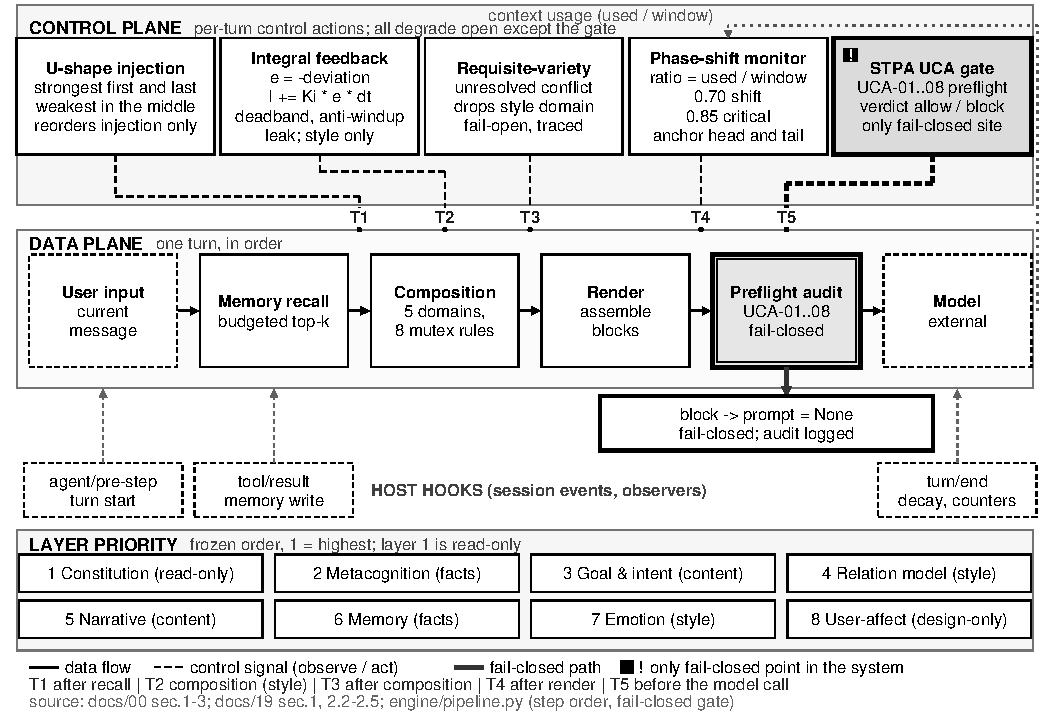
\includegraphics[width=0.98\textwidth]{figures/fig1-architecture.pdf}
\caption{Control plane and data plane. The data plane (lower) is the per-turn
injection path: user message $\rightarrow$ budgeted recall $\rightarrow$
five-domain composition $\rightarrow$ rendering $\rightarrow$ pre-flight audit
$\rightarrow$ external model. The control plane (upper) observes context usage
and acts on the assembly; the STPA gate (shaded) is the \emph{only} fail-closed
site in the system, so a block returns no injectable prompt at all. Dashed lines
are control signals; the layer-priority strip records the frozen precedence
($1$ = highest, layer~1 read-only). Source: \texttt{docs/00} \S1--3,
\texttt{docs/19} \S1--2.5, and the step order in \texttt{engine/pipeline.py}.}
\label{fig:arch}
\end{figure*}

\system{} is a deterministic reference engine (Python, zero model calls) with a
host-side plugin re-implementation. This section specifies eleven mechanisms. Each
subsection follows one template: mechanism semantics, exact code locus
(\texttt{file:line}), then the known defect or cost. All numeric parameters are
design defaults with provenance \texttt{guess}; none is measured
(Section~\ref{sec:limitations}; full table in Appendix~\ref{sec:app:params}).

\subsection{Layering and the single fail-closed point}\label{sec:method:layers}

\paragraph{Mechanism semantics.} Figure~\ref{fig:arch} separates the data plane
(the per-turn injection path) from the control plane that observes and acts on
it. The architecture is an eight-layer,
priority-ordered stack: a read-only constitutional layer constrains every other
layer, and a fixed precedence decides which layer yields first under conflict
in a defence-in-depth order. Exactly one component is
fail-closed---the constitutional
auditor. An empty, malformed, or missing-field proposal is \emph{rejected}
rather than passed, and every other component degrades and logs. A blocked turn
returns no injectable prompt at all.

\paragraph{Code locus.} Layer table and precedence: \texttt{docs/00:11--20};
fail-closed attribution: \texttt{docs/00:68--82}. Auditor with A1--A10 checks and
the C6 blacklist: \texttt{engine/constitution.py:75--117}; empty input and missing
required fields reject at \texttt{engine/constitution.py:83--93}. Frozen-region
hash gate: \texttt{engine/constitution.py:144--177}. The gate closes the pipeline
at \texttt{engine/pipeline.py:181} and \texttt{engine/pipeline.py:205--207}
(\texttt{prompt = None}).

\paragraph{Known defect and cost.} The guarantee is behavioural, not
host-enforced: the constitution is itself text, and plugin configuration is not
protected from replacement by the host. A rejection costs the
whole turn's injection budget (availability traded for safety), and the frozen
hash list ships empty until a freeze command is run.

\subsection{Five-domain composition and mutual exclusion}\label{sec:method:compose}

\paragraph{Mechanism semantics.} Injectable material is partitioned into five
domains---safety, fact, organization, style, retrieval---that act on different
axes and are not ordered against each other. Nine mutual-exclusion rules
resolve pairwise conflicts; an uncovered conflict drops the lower-priority
domain and records \texttt{no\_mutex\_rule}. Assembly order is frozen. Dynamic
domain weights decide only \emph{who is evicted first} when the token budget is
exceeded, never whether a rule fires.

\paragraph{Code locus.} Domain order and mutex table:
\texttt{engine/compose.py:19} and \texttt{engine/compose.py:24--34}; lookup and
application: \texttt{engine/compose.py:43--48}, \texttt{engine/compose.py:79--112};
default policy: \texttt{engine/compose.py:109--112}; weights:
\texttt{engine/compose.py:134--150}; budget eviction:
\texttt{engine/compose.py:180--205}.

\paragraph{Formula.} With indicators for unresolved claims and blocked goals,
and an intensity threshold $\theta_s = 0.6$,
\begin{equation}
w_{\mathrm{fact}} = 0.70 + 0.50\,\mathbf{1}[\mathrm{refuse\_claim}],\quad
w_{\mathrm{org}} = 0.50 + 0.35\,\mathbf{1}[\mathrm{goal\_blocked}],\quad
w_{\mathrm{style}} = 0.40 + 0.40\,\mathbf{1}[\mathrm{intensity} \ge \theta_s].
\end{equation}
Eviction repeatedly removes $\arg\min_b (w_{\mathrm{domain}(b)}, \mathrm{index}(b))$
over soft blocks only; constitution, safety and user blocks are never evicted.

\paragraph{Known defect and cost.} The retrieval domain is never assembled, so
its weight cannot influence eviction. The assumed context length is hardcoded
(8000 tokens, \texttt{engine/compose.py:36}), not drawn from the rule files, and
the budget is never exceeded in replay (utilization $0.137983$), so eviction is
exercised only by unit tests.

\subsection{Dual-channel potency: exponential decay $\cup$ ACT-R base level}\label{sec:method:potency}

\paragraph{Mechanism semantics.} A memory item is ranked by the larger of two
signals: recency-weighted decay (``is it still alive?'') and ACT-R base-level
activation (``is it used often?'')~\cite{anderson1991}. The second channel exists
so that a frequently used but old preference is not archived merely for being
old; the first preserves the frozen baseline ranking.

\paragraph{Formula.} With day-valued access times $t_j$, decay exponent $d$,
offset $\rho$, normalisation bounds $(l,h)$, weight $w$ and type-dependent
half-life $\tau_{\mathrm{type}}$:
\begin{align}
B_i &= \ln\!\Big(\sum_{j \in \text{last }64} (t_{\mathrm{now}} - t_j + \rho)^{-d}\Big),
& n(B_i) &= \mathrm{clip}\!\Big(\frac{B_i - l}{h - l},\,0,\,1\Big),\\
\tau_i^{\mathrm{eff}} &= \tau_{\mathrm{type}(i)}\,(0.5 + \mathrm{imp}_i),
& p_i &= \mathrm{clip}\Big(\max\big(\mathrm{imp}_i e^{-\Delta t_i/\tau_i^{\mathrm{eff}}},\;
w \cdot \mathrm{clip}(\mathrm{imp}_i\, n(B_i),0,1)\big),\,0,\,1\Big),
\end{align}
with $d=0.5$, $\rho=0.001$, $(l,h)=(-3.0,1.0)$, $w=0.6$; a non-positive age
term is replaced by $\rho$, an empty trace yields $B_i=-\infty$, and degenerate
bounds return zero.

\paragraph{Code locus.} \texttt{engine/actr.py:30--41} (base level),
\texttt{engine/actr.py:44--50} (normalisation),
\texttt{engine/actr.py:62--66} (ACT-R potency),
\texttt{engine/memory.py:33--36} (effective half-life),
\texttt{engine/memory.py:39--64} (dual channel). Access traces are written on
recall only when \texttt{memory.touchOnRecall} is enabled
(\texttt{engine/config.py:21}), which is off by default.

\paragraph{Known defect and cost.} The two channels are not commensurable: the
decay term is bounded by importance, while the ACT-R term is bounded by
$w=0.6$, so the $\max$ is an engineering rescue, not a theoretical comparison.
Only base-level activation is implemented---no production rules, buffers,
partial matching or spreading activation---and the ACT-R constants are design
defaults. Replacing decay with pure ACT-R lowered recall on our synthetic
replay set from $1.000$ to $0.556$; this is an internal measurement, not a
replicated result (Section~\ref{sec:problem}). Finally, we do not compute a
rate--distortion functional; the consolidation policy is only analogous to a
rate--distortion trade-off (framing-only, with no code locus).

\subsection{Phase-shift preemptive monitoring}\label{sec:method:phase}

\paragraph{Mechanism semantics.} Context usage is monitored feed-forward. At a
warning ratio the engine raises self-reference and, when the trend is rising or
a hard ratio is crossed, clamps a persona anchor around the prompt; it does not
wait for observed degradation.

\paragraph{Formula.} For usage $u$ and window $W$,
\begin{equation}
r = \begin{cases}
0, & W \le 0 \quad \text{(no history update, phase unknown)}\\
\max(0, \min(r_{\max}, u/W)), & W > 0
\end{cases}
\qquad
\phi = \begin{cases}
\text{critical}, & r \ge \alpha_h\\
\text{shift}, & \alpha_s \le r < \alpha_h\\
\text{normal}, & r < \alpha_s
\end{cases}
\end{equation}
with $\alpha_s=0.70$, $\alpha_h=0.85$, $r_{\max}=1.5$, history capacity $64$, and
trend $\tau_t = (r_t - r_{t-2})/2$ when at least three samples exist. Then
$\mathrm{prefeed} = \phi \ne \text{normal}$, and
$\mathrm{anchor\_required} = (\phi = \text{critical}) \lor
(\phi = \text{shift} \land \tau_t > 0.02)$.

\paragraph{Code locus.} \texttt{engine/control.py:78--123}; the hard branch is
tested before the warning branch at \texttt{engine/control.py:103--109} (an
earlier ordering made critical unreachable). Observation is wired at
\texttt{engine/pipeline.py:118--121} and is skipped unless the caller supplies
both counts. Anchoring: \texttt{engine/control.py:130--138},
\texttt{engine/pipeline.py:159--162}.

\paragraph{Known defect and cost.} The dual trip points are not hysteresis: there
is no falling-edge threshold, and the two points carry different meanings
(warning vs. mandatory). The trend term spans two samples, not one, so a spike
is compared against a two-step baseline. Usage is estimated from characters, not
tokens, so absolute ratios are not comparable to a tokenizer, and engine-mode
runs cannot evidence real degradation. Both thresholds are design defaults.
Finally, since $\mathrm{anchor\_required} \Rightarrow \mathrm{prefeed}$, the
second flag is a modality label rather than an independent trigger.

\subsection{Requisite-variety dimensionality reduction}\label{sec:method:variety}

\paragraph{Mechanism semantics.} When a conflict is unresolved and no
mutual-exclusion rule covers it, the controller shrinks its own action space
instead of improvising: it drops the style domain and renders neutral facts plus
an explicit clarification marker~\cite{ashby1956}. The gate is fail-open---the
verdict stays \texttt{allow} and only the injected content is reduced.

\paragraph{Code locus.} Guard and marker: \texttt{engine/control.py:143--170};
pipeline wiring: \texttt{engine/pipeline.py:147--154}; actual removal and
drop accounting: \texttt{engine/pipeline.py:239--251}. The condition is
$\mathrm{fallback} = \mathbf{1}[\mathrm{conflict} = \texttt{unresolved} \land
\neg \mathrm{matched\_mutex}]$.

\paragraph{Known defect and cost.} The engine has no conflict detector. The
pipeline obtains the conflict label from the metacognitive verdict, which is
called without that argument and therefore returns \texttt{none}
(\texttt{engine/pipeline.py:105}; \texttt{engine/metacog.py:45--47}), and it
hardwires \texttt{matched\_mutex = False} (\texttt{engine/pipeline.py:150}).
Consequently the reduction path is unreachable during replay and can only be
exercised when a caller supplies the label. The plugin adds a rule-based
detector, but that is a rule stub with no measured error rate. Only one domain
is ever dropped; the guard quantifies no variety.

\subsection{Causal interposition safety gate over unsafe control actions}\label{sec:method:gate}

\paragraph{Mechanism semantics.} After assembly and rendering, and before any
model call, a checklist of unsafe control actions (UCAs) audits the candidate
injection~\cite{leveson2018}. Any hit in UCA-01--07 blocks the turn; UCA-08
(integrating past a saturated baseline) is downgrade-only and must not change
the verdict.

\paragraph{Formula and code locus.} With the candidate prompt $p$, fact block
$f$, and saturation flags $s_k$,
\begin{equation}
\begin{aligned}
H_1 &= \exists\, w \in W_{\mathrm{override}}:\ w \subseteq p, &
H_2 &= \neg \mathrm{frozen\_ok}, &
H_3 &= \mathrm{refuse} \land \mathrm{style\_injected},\\
H_4 &= \exists\, w \in W_{\mathrm{unsourced}}:\ w \subseteq f, &
H_5 &= \neg \mathrm{constitution\_injected}, &
H_6 &= (\mathrm{conflict} = \texttt{unresolved}) \land \neg \mathrm{fallback\_applied},\\
H_7 &= \mathrm{prefeed} \land (\text{anchor marker} \not\subseteq p), &&
\end{aligned}
\end{equation}
$\mathrm{verdict} = \texttt{block}$ iff $\bigvee_{i=1}^{7} H_i$, while
$\mathrm{downgrades} = [\texttt{UCA-08}]$ iff $\exists k: s_k$. Checks follow
code order; the UCA-03 predicate is narrowed to
$H_3 \land \neg\,\mathrm{soft\_buffer\_applied}$ when a soft buffer is recorded
(Section~\ref{sec:method:immersive}); both word lists and the eight-row UCA table
are hardcoded at
\texttt{engine/control.py:175--188} (full table in
Table~\ref{tab:uca}); the gate is
\texttt{engine/control.py:191--232}; invocation and the fail-closed exit are
\texttt{engine/pipeline.py:165--180} and \texttt{engine/pipeline.py:205--207}.

\paragraph{Known defect and cost.} The gate scans only the assembled injection
text. Because assembled blocks are fixed templates that contain no user text
(\texttt{engine/compose.py:157--177}), engine-side user-turn jailbreaks cannot
fire it; user-message scanning exists only in the plugin and cannot remove the
message from the host payload. Detection is lexical with no coverage estimate,
\texttt{fail\_mode} is a constant label rather than a mode switch, and
saturation must be supplied by the caller (\texttt{engine/pipeline.py:91})---the
integral controller and this gate are not internally connected. Our 24-sample
jailbreak corpus is constructed to contain the trigger phrases, so its 24/24
block rate is a wiring check, not a robustness result.

\subsection{Immersive Safety: A Decoupled Refusal Surface}\label{sec:method:immersive}

\paragraph{Mechanism semantics.} Two existing paths turn a safety decision into a
persona collapse. A gate block (Section~\ref{sec:method:gate}) leaves the plugin
with a constitution fragment and a terse system-break notice; requisite-variety
reduction (Section~\ref{sec:method:variety}) drops the style domain when a
conflict is unresolved. Both are defensible for safety, and neither is changed
here. The cost is coupling: the factual refusal and the expressive surface are
one switch, so a mild role-play probe that could be refused in character instead
silences the character. In role-play and companion deployments this converts a
safety event into an experience failure. We describe this as a coupling cost, not
as a safety benefit, and we do not claim that the previous behaviour was unsafe.

The decoupling adds a ninth mutual-exclusion rule: the soft buffer. Rule~8 is
unchanged---a hard reject still drops style, organization and retrieval. Rule~9
applies only when the gate's severity is soft: the style domain is retained but
constrained to a warning/confused micro-expression drawn from the engine's
existing closed label set (we adopt PAD~\cite{mehrabian1974} as the interpretive
frame; no labels are added), the intensity is capped at
\texttt{softBufferMaxIntensity} $=0.45$, and the relation modifier is clamped to
$[0.8,1.0]$ so that a safety buffer cannot amplify intimacy. Fact, organization
and retrieval stay dropped. The factual refusal instruction remains mandatory and
enters the context as \texttt{[System\_Notice: Safe\_Redirect]}, so compliance is
still refused: the model may not execute the request, may not offer a workaround,
and is limited to a two-sentence in-character refusal.

\paragraph{Risk tiers and escalation.} Classification is a pure lexical function
of the user turn and the relation's trust level---rule stubs, not a model:
\texttt{classify\_user\_risk} returns \texttt{none}, \texttt{mild} or
\texttt{severe}~\cite{leveson2018}. \texttt{mild} (role-play framing together
with a risk term) maps to a soft block; \texttt{severe} (explicit override, a
bypass request, or a red-line category) maps to the existing hard block;
\texttt{none} leaves the v3.0 path untouched. Consecutive non-exempt
\texttt{mild} hits escalate to a hard block after \texttt{escalateAfterSoftHits}
$=3$ (a design default), with the streak persisted in host state so that a fresh
process cannot reset it, and any \texttt{none} turn resets it. A trust exemption
is narrower still: it requires \texttt{mild}, a harmless joke, and high trust
simultaneously; \texttt{severe} is never exempt.

\paragraph{Invariants.} Fail-closed is unchanged. A hard turn still returns
\texttt{prompt=None} with the neutral notice, and a soft turn keeps
$\mathrm{verdict}=\texttt{block}$; the only prompt allowed in the soft case is the
constrained redirect text. The gate's UCA-03 predicate is narrowed to
$\mathrm{refuse} \land \mathrm{style\_injected} \land
\neg\,\mathrm{soft\_buffer\_applied}$: unconstrained style injection in a refusal
scene still counts, the constrained buffer does not, and the soft turn is still
blocked under UCA-01 from the user message. With
\texttt{immersiveEnabled}$=$\texttt{false}, or when no risk is detected, the
composition, audit and pipeline outputs are byte-identical to v3.0 by
construction.

\paragraph{Code locus and evidence.} Classification and intervention decisions:
\texttt{engine/control.py} (\texttt{classify\_user\_risk},
\texttt{decide\_intervention}) and the plugin port in
\texttt{plugin/dsh-lingshu/control.js}; rule~9 and the constrained re-mount:
\texttt{engine/compose.py}; tier wiring and the blocked-severity event field:
\texttt{engine/pipeline.py}; host-side rendering and the persisted streak:
\texttt{plugin/dsh-lingshu/index.js}. Evidence is assertion-level only:
\texttt{tests/test\_immersive\_safety.py} covers classification, the soft
composition path, clamping, escalation, the trust exemption and the default
zero-regression case; \texttt{plugin/dsh-lingshu/host-sim.mjs} and
\texttt{plugin/dsh-lingshu/control-sim.mjs} add the corresponding mock-host
assertions. One real-host mild jailbreak is reported in the accompanying
acceptance report (\texttt{acceptance/immersive-safety-host-2026-10-27.md}): $n=1$,
model output is stochastic, and the lexical word lists have no calibrated
false-positive rate. The evidence establishes that the mechanism is reachable in
the tested configuration; it establishes no user-experience gain, and no user
study was run.

\paragraph{Known defect and cost.} The buffer is a lexical rule stub: its
false-positive and false-negative rates are uncalibrated, and the label set is
small enough that a retained micro-expression may read as generic. Keeping style
in a refusal scene also keeps a negotiation surface; the prompt constraints are
designed to bound it, but their effect is untested here. The escalation
threshold and the intensity cap are design defaults with provenance
\texttt{guess}. Finally, the construction depends on the host actually rendering
the constrained style and the redirect notice; in engine-only mode the path is
exercised by tests alone.

\subsection{U-shaped attention anchoring}\label{sec:method:ushape}

\paragraph{Mechanism semantics.} Retrieval order and injection order are
separated. The highest-scoring item goes first, the second-highest last, and the
weakest items occupy the middle, on the hypothesis that prompt boundaries are
better attended than the middle.

\paragraph{Formula and code locus.} For $n>2$ and a score-descending list
$[r_0,\dots,r_{n-1}]$, $\mathrm{out} = [r_0,r_2,r_4,\dots] \Vert
([r_1,r_3,\dots])^{\mathrm{rev}}$; $n \le 2$ is identity. Hence
$n=3 \rightarrow [r_0,r_2,r_1]$ and $n=5 \rightarrow [r_0,r_2,r_4,r_3,r_1]$.
\texttt{engine/pipeline.py:43--61}; the permutation is applied to the injection
field only (\texttt{engine/pipeline.py:102}, \texttt{engine/pipeline.py:196}) and
the retrieval return order is untouched.

\paragraph{Known defect and cost.} Membership is unchanged, so the mechanism can
only matter through a model's position bias, which the zero-model engine cannot
measure. The rationale is external to this work and untested here, and with
$n \le 2$ the permutation is the identity.

\subsection{Integral feedback with anti-windup}\label{sec:method:integral}

\paragraph{Mechanism semantics.} Sustained negative affective deviation moves a
baseline rather than conceding one turn, with three engineering constraints:
deadband (leak only, do not integrate), anti-windup (stop integrating once the
cap is reached, standard practice~\cite{astrom2006}) and leakage (return to
zero after the user recovers).

\paragraph{Formula.} For each dimension and elapsed time $\Delta t = \max(0,
\mathrm{dt})$:
\begin{equation}
I_k \leftarrow
\begin{cases}
I_k e^{-\lambda \Delta t}, & \lvert e_k \rvert < \varepsilon\\
I_k e^{-\lambda \Delta t}, & e_k < 0\\
I_k e^{-\lambda \Delta t}, & s_k = \mathrm{true}\\
\mathrm{sat}(I_k + K_i e_k \Delta t), & \text{otherwise}
\end{cases}
\qquad e_k = -\delta_k,
\end{equation}
where $\mathrm{sat}(x) = \mathrm{sign}(x)\,C$ and $s_k \leftarrow
\mathrm{true}$ if $\lvert x \rvert \ge C$, and $\mathrm{sat}(x)=x$ otherwise;
$K_i=0.15$, $C=0.4$, $\lambda=0.05$, $\varepsilon=0.02$. The baseline is $I_k$.

\paragraph{Code locus.} \texttt{engine/control.py:30--73} (class, step and
application), with parameters in \texttt{rules/decay-params.yaml:224--227}.

\paragraph{Known defect and cost.} This is a one-sided (rectified) leaky
integrator, not a textbook PI controller: positive deviation never raises the
baseline. Saturation is a latch---the flag is never reset, so after saturation
the dimension only leaks---and there is no plant model, no stability argument
and no calibration: all four gains are design defaults. The controller is not
wired to the gate; UCA-08 is observable only when a caller passes the flags.

\subsection{Learning loop: measure, propose, verify}\label{sec:method:learn}

\paragraph{Mechanism semantics.} Learning produces proposals, never direct
edits. A correction is rewritten into a new test sample, a candidate knob is
replayed, and a proposal is emitted only if the correction is resolved, the
objective does not regress, and guardrails hold; proposals remain
non-deployable unless an independent red-team pass is recorded.

\paragraph{Code locus.} Deterministic replay with fixed clock, scoring and
single-parameter attribution: \texttt{engine/replay.py:39--151}. Evidence gate,
candidate knobs and the blacklist: \texttt{engine/proposal.py:24--49},
\texttt{engine/proposal.py:103--197}. Guardrail thresholds and rollback classes:
\texttt{engine/gray.py:17--45}, verdict at \texttt{engine/gray.py:63}. The
significance floor is $0.02$ and the evidence floor is three same-kind
corrections; targets under evaluation, replay-set, guardrail, constitution or
composition scope are rejected outright.

\paragraph{Known defect and cost.} Learning is disabled by default
(\texttt{rules/learning-params.yaml:10}); levels above parameter search are
unimplemented, and no proposal is ever applied automatically. The search space
is tiny, the corpus is synthetic, and the one completed grid search found no
materially better configuration---so the honest claim is that the loop is
executable and auditable, not that it improves anything.

\subsection{Reference engine and host plugin}\label{sec:method:port}

\paragraph{Mechanism semantics.} The engine is a reference implementation; the
plugin re-implements the same semantics in the \host{} host process, to avoid
turning pure computation into inter-process I/O.

\paragraph{Code locus.} Engine-side originals:
\texttt{engine/control.py:30--73} and \texttt{engine/actr.py:30--66}. Plugin
classes mirroring the engine:
\texttt{plugin/dsh-lingshu/control.js:83} (integral),
\texttt{plugin/dsh-lingshu/control.js:155--172} (phase monitor),
\texttt{plugin/dsh-lingshu/control.js:208--216} (anchoring),
\texttt{plugin/dsh-lingshu/control.js:236} (variety guard),
\texttt{plugin/dsh-lingshu/control.js:282} (U-shaped order),
\texttt{plugin/dsh-lingshu/control.js:296--362} (UCA table, gate and the
user-message scan). Known divergences are tabulated at
\texttt{docs/19:191--222}; numeric parity across rule file, host patch and
plugin defaults is machine-compared for 66 keys.

\paragraph{Known defect and cost.} Anchors are injected as two host sections
(true head/tail wrapping is not available), usage is estimated from characters,
refusal is never set by the plugin (so UCA-03 is unreachable there), and dynamic
weights are not ported. Plugin evidence consists of mock-host assertions
(188 + 148 + 45 + 15 = 396), not real traffic.

\section{Experiments}\label{sec:experiments}

We report an executable artefact, a deterministic zero-model ablation with
pre-registered hypotheses, and an illustrative real-host pilot.

\subsection{Artifact and reproducibility}\label{sec:exp:artifact}

The engine is zero-dependency Python with no model calls; the plugin is a
JavaScript re-implementation. Feasibility is asserted: 892 Python assertions over
14 test files and 396 plugin assertions (188/148/45/15), the latter count taken
at the 2026-10-27 audit snapshot and not re-executed for this paper. Re-executed
here for
Section~\ref{sec:method}: 161, 65 and 26 assertions, all pass. Three drift
checks were green at submission: a 66-key rule/engine/plugin comparison, a
contract digest, and an implementation-status matrix check. Determinism is
enforced: fixed clock (60\,s per turn), no wall clock, no randomness, no
network. Same configuration, store and script give byte-identical runs; this run
reports \texttt{model\_calls=0}, \texttt{network\_calls=0}, two written files and
51/51 verifier checks.

\subsection{Deterministic three-arm ablation}\label{sec:exp:ablation}

\paragraph{Protocol.} A 100-turn script is generated deterministically from the
chaos and replay corpora (SHA-256 \texttt{701ff06a0b37\ldots}): 21,610 characters
against a 24,000-character window, maximum usage ratio $0.9004$, with the
phase-shift monitor firing on turns 73--100 (28 turns). Twelve probes cover
long-range settings (A), superseded values (B), distractor-overloaded settings
(C), and a constructed high-frequency-old preference (D, 30 accesses ending 100
days ago); two no-hit probes sit at turns 86--87. Hits are decided by entry
sensitivity. \textsc{Baseline} injects the last three raw turns with no memory or
control layer; \textsc{Basic} uses budgeted query-conditioned recall with the
ACT-R channel off (\texttt{actrWeight=0}), static weights and no control layer;
\textsc{Full} uses defaults, i.e.\ both potency channels, dynamic weights and all
four control subsystems. Harness and pipeline agree on 100/100 turns for the
wire-compatible core; label-on divergences are recorded in the result file.
Table~\ref{tab:ablation} and Figure~\ref{fig:retention} report the outcomes.

\begin{table*}[t]
\centering\footnotesize
\caption{Three-arm ablation. SFR: setting-forgetting rate per class and overall;
NHD: no-hit discipline (literal variant in parentheses); IIR: adversarial
interference ratio; telemetry: phase/anchor turns, fallback marks (actual drops),
UCA-08 records. Source:
\texttt{results/abl-20261027-003626-engine.json}, fields
\texttt{conditions.<arm>.metrics.*} and \texttt{conditions.<arm>.telemetry.*};
verifier 51/51.}
\label{tab:ablation}
\begin{tabular}{@{}l cccc c c c c c ccc c@{}}
\toprule
 & \multicolumn{4}{c}{SFR by probe class} & & & & & & \multicolumn{3}{c}{Jailbreak (\%)} & \multicolumn{1}{c}{Telemetry}\\
\cmidrule(lr){2-5}\cmidrule(lr){11-13}\cmidrule(lr){14-14}
Arm & A & B & C & D & SFR$_{\text{text}}$ [95\% CI] & SFR$_{\text{id}}$ & IIR & NHD & UCE & in & fp & script & ph/anc/fb/08 \\
\midrule
Baseline & 1.00 & 1.00 & 1.00 & 1.00 & 1.00$^{\ddagger}$ & $\varnothing$ & $\varnothing$ & $\varnothing$ & $0^{\dagger}$ & $\varnothing$ & $\varnothing$ & $\varnothing$ & 0/0/0/0 \\
Basic & 0.00 & 0.00 & 0.00 & 1.00 & 0.25 [0.05, 0.57] & 0.25 & 0.56 & 1.00 (0.00) & $0^{\dagger}$ & $\varnothing$ & $\varnothing$ & $\varnothing$ & 0/0/0/0 \\
Full & 0.00 & 0.00 & 0.00 & 0.00 & 0.00 [0.00, 0.26] & 0.00 & 0.47 & 1.00 (0.00) & $0^{\dagger}$ & 1.00 (25) & 0.00 (294) & 0.00 (6) & 28/28/4(0)/62 \\
\bottomrule
\end{tabular}

\vspace{2pt}
\raggedright\scriptsize
$\varnothing$: not applicable; the cell is \texttt{null} with a reason, never
zero. $^{\ddagger}$: by construction---a three-turn window cannot contain a
setting planted 85 turns earlier. $^{\dagger}$:
structurally zero, since all injected items are active and user-explicit.
\end{table*}

\paragraph{Results.} Both LINGSHU arms retrieve the nine A/B/C probes perfectly,
and the baseline's $1.00$ is window arithmetic---definitional by construction---so
we do not treat the baseline--system difference as an effect size. The arms separate only on class D:
\textsc{Basic} misses all three, \textsc{Full} retrieves all three, giving $0.25$
versus $0.00$ ($p=0.125$, three discordant pairs, not significant). With twelve
paired probes the exact sign test detects only a $5/12\approx0.42$ difference at
$\alpha=0.05$ ($6/12=0.50$ after Bonferroni correction), and a three-item class
cannot reach significance at all; we therefore report direction and per-probe
detail only. Order permutations leave SFR unchanged but move anchor counts
(28/62/21): retention is order-robust, phase timing is not.

Pre-registered outcomes are reported with failures. P1b passes on its point
estimate but fails its confidence criterion (Basic's Clopper--Pearson upper bound
is $0.572$ against a required $0.45$). P2 passes under the code-faithful
predicate, while the literal substring predicate returns $0.00$ because the
engine's wording differs; both numbers stand. P3 is not evaluable, as both arms
are structurally zero. P5 is undecidable:
in-distribution jailbreaks are blocked 25/25, false positives are 0/294 and
scripted user-turn jailbreaks 0/6, but the held-out set was never
authored, so that cell is \texttt{null}. P6 passes (28 phase turns, 28
anchors, 4 fallback marks, 62 UCA-08 records for \textsc{Full}; all zero for
\textsc{Basic}). P7 passes for single-anchor overhead ($+100$ to $+124$
characters) but fails its literal two-times threshold.

\paragraph{Reading the phase window.} Both thresholds fall inside the run: the
ratio crosses $0.70$ at turn 73 (phase \emph{shift}) and $0.85$ at turn 85 (phase
\emph{critical}), so the shift window is turns 73--100 and the critical window
turns 85--100 (Section~\ref{sec:method:phase}). The telemetry shows what the
thresholds change in practice, not only in the formula: \textsc{Full} records 28
phase turns and 28 anchors with 4 fallback marks and 62 UCA-08 records, while
\textsc{Basic} records 0/0/0/0, and the anchor strip under Figure~\ref{fig:retention}
begins at turn 73 and continues through the critical window. The figure also shows
why the phase monitor cannot improve retention by itself: \textsc{Basic} and
\textsc{Full} have identical injected sets, so the shaded bands mark when the
control plane starts paying a prompt-budget cost, not when memory improves. We
therefore read the 70\%/85\% thresholds as escalation points for anchoring and
audit, not as learning or retrieval gains.

\subsection{Real-host pilot}\label{sec:exp:host}

Ten cells ran on one host and one model route, one run each. The details are in
Appendix~\ref{app:hostpilotdata}; the methodological finding is that compressing
a 100-turn dialogue into one 78\,KB request dilutes the query until
query-conditioned retrieval stops hitting (\textsc{Full} reports \texttt{matched=0}),
and the control layer never fired in any cell (the gate returned \texttt{allow}
with an empty UCA list throughout). This is a mechanism demonstration at $n=1$,
not a hallucination rate.

\begin{figure*}[t]
\centering
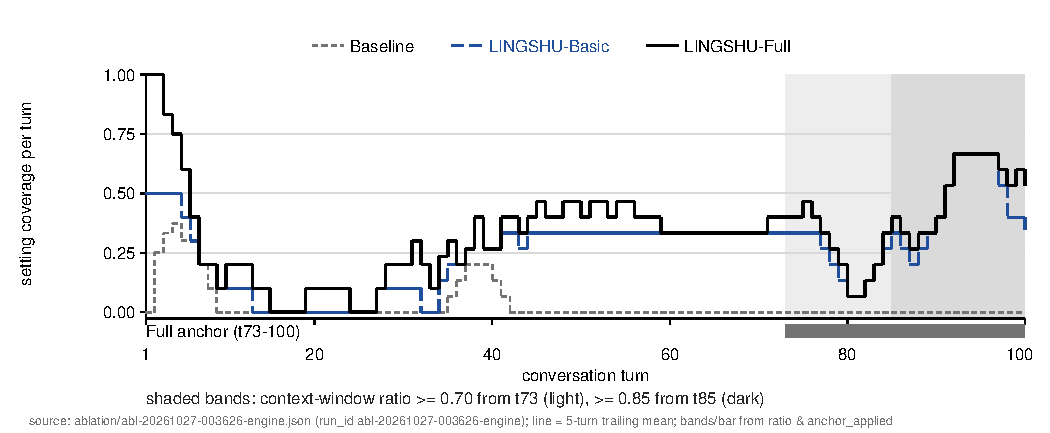
\includegraphics[width=\textwidth]{figures/fig2-retention.pdf}
\caption{Setting coverage per turn over the 100-turn script:
$y_t = |\mathcal{S}^{\mathrm{inj}}_t \cap \mathcal{S}^{\mathrm{act}}_t| /
|\mathcal{S}^{\mathrm{act}}_t|$, the fraction of currently active planted
settings that appear in the injected context (plotted as a 5-turn trailing mean;
the raw turn means are 0.025, 0.260 and 0.327 for
Baseline, Basic and Full). Basic and Full overlap by design: the control plane
does not change retrieval membership. Shaded bands mark the phase-shift window
($r \ge 0.70$ from turn 73, $r \ge 0.85$ from turn 85); the strip below the axis
marks turns on which Full injects head/tail persona anchors. Source:
\texttt{conditions.<arm>.turns[].\{setting\_ids\_injected, active\_setting\_ids,
ratio, anchor\_applied\}} in \texttt{abl-20261027-003626-engine.json}.}
\label{fig:retention}
\end{figure*}

\subsection{Robustness under Chaos Injection}\label{sec:exp:chaos}

\paragraph{Protocol.} Three faults are injected from \emph{outside} the system;
\texttt{plugin/}, \texttt{engine/} and \texttt{rules/} are hashed before and
after the campaign and are unchanged. Each case runs in its own \texttt{DSH\_HOME}
whose profile copy links (via a directory junction) to the repository plugin, so
the measured code is the current reference implementation and the injection is
confined to the host layer and to on-disk memory state. All runs are headless CLI
invocations with a fixed short prompt; transcripts, plugin state, audit logs and
final prompts are written to disk and analysed offline. One injected point is run
once ($n=1$); no red-team mutation is performed in this section.

\emph{A, transport faults.} The host's model endpoint is redirected through the
documented \texttt{DEEPSEEK\_BASE\_URL} environment variable to a local mock that
returns HTTP 500, a valid but empty 200 response, a valid 200 response carrying a
fabricated answer, or accepts the connection and never answers.

\emph{B, memory faults.} The memory store is corrupted at the file level, without
touching \texttt{memorywriter.js}: (B1) \texttt{memory.jsonl} is replaced by a
directory, so reads fail with \texttt{EISDIR} and are swallowed while writes throw;
(B2) a readable but dirty store is seeded with a torn JSON line, a duplicate id
whose later row is a supersession tombstone, and two active rows that share
$(\textsc{subject},\textsc{relation})$ but disagree on \textsc{object}. A warm-state
template is pre-seeded so that the cold-start gate does not mask the effect; this
setup is synthetic and disclosed as such.

\emph{C, context flood.} A deterministic 150{,}000-character garbage stream
($\approx 50$k tokens at the plugin's 3-chars/token estimator) is passed as the
user message while \texttt{LINGSHU\_CONTEXT\_WINDOW} fixes the plugin's perceived
window at four values; a mock endpoint records the assembled request body, so the
run costs no model tokens.

\begin{table*}[t]
\centering\footnotesize
\caption{Fault-injection matrix. Every cell is an observed value from one run;
$\varnothing$ marks a quantity the injected fault makes inapplicable, never zero.
A: five transport modes on one fixed prompt. B: three headless runs on a synthetic
warm state. C: four window values on the same 150k-character input plus exact
boundary brackets. Source: \texttt{experiments/chaos-injection/out/}.}
\label{tab:chaos}
\begin{tabular}{@{}l l l l@{}}
\toprule
Fault & Injected mode & Control-plane observation & Key numbers \\
\midrule
A transport & HTTP 500 & error surfaced by host; injection still ran once & 7 tries, 17.99 s, exit 1 \\
            & empty 200 & empty final message passed through, exit 0 & final length 0 \\
            & fabricated 200 & fabricated text reached stdout, exit 0 & final length 23 \\
            & never answers & no client-side timeout inside 150 s window & $\ge$150.03 s \\
            & all modes & \texttt{blocked=false}; constitution in prompt & 5/5 \\
B memory    & store as directory (B1) & \texttt{hook\_error}=1 (\texttt{EISDIR}); writes 0; reply returned & 9.851 s, exit 0 \\
            & dirty store (B2) & \texttt{fallback=true}, \texttt{drop style}; superseded not recalled & 21.046 s, exit 0 \\
            & clean control (B0) & style and organization injected; no fallback & 45.654 s, exit 0 \\
C context   & 4 windows, 150k chars & \texttt{normal/shift/shift/critical}; constitution 4/4 & ratios 0.681/0.701/0.721/0.851 \\
            & boundary brackets & \texttt{0.7000}$\to$normal, \texttt{0.7006}$\to$shift; \texttt{0.8500}$\to$shift, \texttt{0.8507}$\to$critical & 8 headless calls, 0 model calls \\
\bottomrule
\end{tabular}
\end{table*}

\paragraph{Transport faults (A).} A plain 200 response completes in 2.84\,s. An
HTTP 500 is retried by the host seven times with exponential backoff
(0.55, 0.96, 1.92, 4.25, 7.51\,s between attempts) and surfaces one error line
(\texttt{dsh: SERVER: mock upstream 500}) after 17.99\,s, exiting non-zero with
\emph{no} fabricated text. An endpoint that never answers produces no response
within a 150\,s observation window and is terminated by the harness, not by a
client timeout. In all five modes the plugin performed exactly one pre-step
injection, the constitution section remained in the final prompt,
\texttt{state.control.blocked} stayed false and no hook error was recorded. An
empty 200 response was passed through as an empty final message (exit 0), and a
fabricated 200 response reached stdout verbatim (23 characters). The control plane
therefore never converts a transport failure into fabricated content, but it adds
neither a transport timeout nor an output validator: those remain host-layer
responsibilities.

\paragraph{Memory faults (B).} With a clean store (B0) the injected prompt carries
constitution, metacognition, organization and style sections and no fallback mark.
Replacing the store by a directory (B1) raises one \texttt{hook\_error}
(\texttt{Error: EISDIR ... write}) and leaves \texttt{stateWrites} at its
pre-run value, yet the turn still exits 0 and returns a 364-character answer with
the constitution and style sections intact---feature fail-open, memory isolated.
Two caveats are reported rather than smoothed over: the reply asserts that the
fact was recorded although the write demonstrably failed, and the model's
own status narration quotes the synthetic warm-template counter, so only on-disk
evidence is used for judgement. With the dirty store (B2) recall returns
\texttt{mem\_002} and \texttt{mem\_003} while the superseded tombstone
\texttt{mem\_001} is absent; the conflict on the
$(\textsc{subject},\textsc{relation})$ pair is classified
unresolved, the variety guard sets \texttt{fallback=true} with
\texttt{dropDomains=["style"]}, the final prompt loses its style section but keeps
the conflict-to-clarify marker and the constitution block, \texttt{verdict} remains
\texttt{allow} and \texttt{blocked} false, and the model asks the user to
disambiguate instead of choosing a value. The dirty store also exposes a
rule-stub artefact: the \emph{question} ``what is my project codename?'' is
extracted as a fact whose object is the interrogative ``what'', and in B2 its
write supersedes both conflicting rows
(\texttt{supersedeEvents}=2). That artefact must not be read as a benefit: it
means the next turn's conflict can be erased by the query itself.
\footnote{The byte-exact CJK prompt markers and conflict keys are recorded
verbatim in \texttt{experiments/chaos-injection/out/}; this paper renders them in
ASCII so that the source compiles with the standard T1 fonts.}

\paragraph{Context flood (C).} Measured usage ratios (four decimals) are 0.6806,
0.7006, 0.7206 and 0.8507 for the four windows; the phase is
\texttt{normal}, \texttt{shift}, \texttt{shift}, \texttt{critical} respectively.
Two exact boundary brackets pin the thresholds: under $\ge$ semantics the largest
shifting window is 71{,}490 ($r=0.700000$), and 71{,}491 is \texttt{normal};
the largest critical window is 58{,}874 ($r=0.8500017$) and 58{,}875 is
\texttt{shift}. Four-decimal display is a trap: window 71{,}493 prints
\texttt{0.7000} yet stays \texttt{normal}, and 58{,}876 prints \texttt{0.8500}
yet stays \texttt{shift}; only the unrounded ratio is decisive. The plugin's
estimate is 50{,}043 tokens for a nominal 50{,}000: its input is the 150{,}127-character
JSON message envelope (127 characters of \texttt{role}/\texttt{content} wrapping),
so all measured ratios sit $\approx 0.0006$ above their nominal values. The host
then renders 151{,}936 JSON characters (50{,}646 tokens), appending a
1{,}809-character instruction block to the user message; the plugin therefore
under-estimates model-visible input by about $1.2\%$. Physical occupancy is
$\approx 5.2\%$ of the model's 1M-token window: the window here is a laboratory
override, and the ratio is a relative control signal rather than a saturation
measurement.

No truncation occurs: in 4/4 runs the full input appears in the mock request body
(\texttt{prompt\_full\_in\_body}), the truncation rate is 0.0, and the constitution
section is present in 4/4 requests. Anchor delivery, however, exposes a genuine
one-assembly lag. The plugin's own prompt preview carries a head anchor whenever
\texttt{prefeed} is set and both head and tail anchors once \texttt{critical};
the \emph{request} reaching the model carries the anchor set of the \emph{previous}
turn in 8/8 observed requests. The clearest case is the first \texttt{critical}
turn: its preview has head and tail, its request has only the head, and only the
next request carries both. The mechanism is host-side: the agent loop assembles the
system prompt before it emits \texttt{agent/pre-step}, where the plugin updates the
phase state (assembly precedes the hook by four source lines in
\texttt{dsh-agent-loop}); the plugin cannot rewrite the already-composed request.
Even when delivered, the tail anchor ends at system offset 229 of 2{,}906 characters,
i.e.\ at roughly $0.17\%$ of the model-visible text, so ``head and tail'' means
sections 90/140 of the plugin's seven-part prompt, not the absolute ends of the
request. A single-turn or single-shot deployment should therefore not expect
critical anchors to take effect on the turn that produces the critical ratio.

\begin{figure*}[t]
\centering
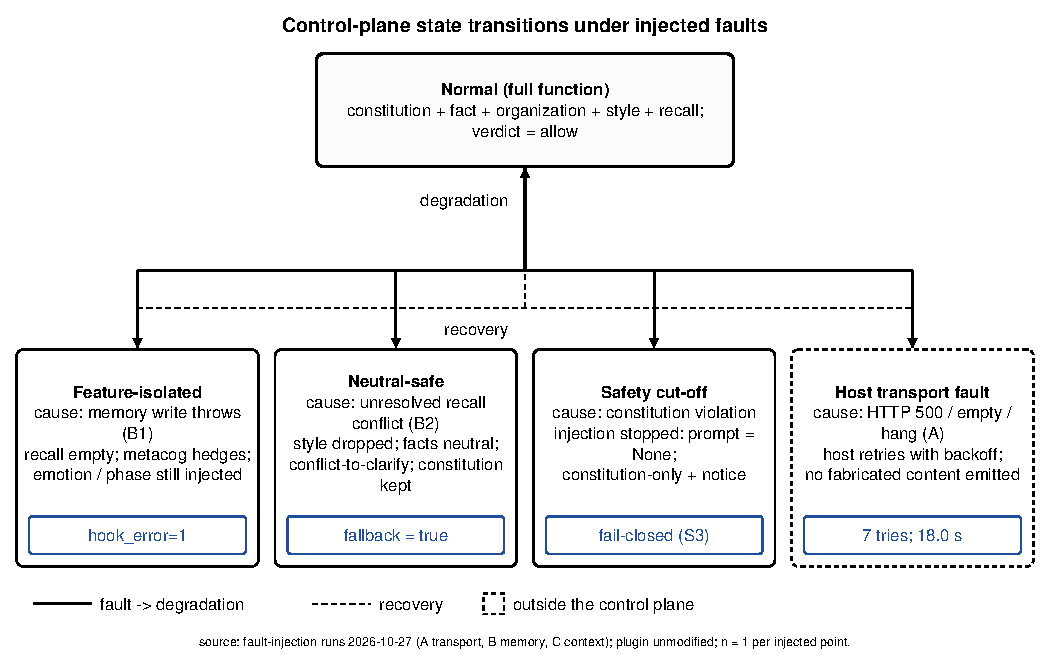
\includegraphics[width=0.98\textwidth]{figures/fig3-robustness.pdf}
\caption{Control-plane state transitions under injected faults. Normal operation
degrades along three distinct paths---feature isolation under a memory write
failure (B1), neutral-safe output under an unresolved recall conflict (B2), and
the security cut-off under a constitution violation (the existing STPA evidence
in \texttt{docs/22})---while transport faults remain outside the control plane
(A). Solid arcs are fault-to-degradation transitions, dashed arcs are recoveries.
Per-point evidence and the exact numbers are in
\texttt{experiments/chaos-injection/out/}; $n=1$ per injected point, plugin
unmodified.}
\label{fig:chaos}
\end{figure*}

\paragraph{What the asymmetry guarantees.} Across the three scenarios the control
plane behaves asymmetrically in exactly one direction: when a \emph{security}
predicate is at stake the gate is fail-closed and stops injection rather than
softening refusal, while when a \emph{feature} is at stake the failure is
fail-open---memory isolation and neutral-safe output keep the turn usable, the
constitution block is preserved and no fault is silently converted into
content---so \emph{LINGSHU's asymmetric degradation mechanism (fail-closed for
security, fail-open for features) ensures system availability under extreme
chaos}. The scope of that sentence is the control plane. Transport faults are
surfaced but neither timed out nor retried by the plugin, model output is not
validated by the plugin, and one B1 reply asserted a persistence that did not
happen; availability under transport faults therefore depends on the host, and
output truthfulness remains outside the mechanism's remit.

\subsection{Scope of the evidence}\label{sec:exp:notshow}

These experiments establish contract behaviour and mechanism reachability, not
model-level effect sizes: the engine is model-free, the host runs are one run per
cell on one model route, and the chaos faults are $n=1$ synthetic injections
rather than a sample of production failures. Two structural limits are worth
naming here because they shape the claims: the anchor set that reaches the model
lags the plugin's phase by one assembly, so the first critical request carries
only the head anchor; and host runs involve a real model and are therefore not
deterministic, which is why every claim above is tied to a field in the evidence
files rather than to a summary sentence. The full itemised list of parameter,
sample and environment limits is consolidated in Section~\ref{sec:limitations}.

% 06b-supplement.tex - supplementary Results subsections (S1 mechanism ablation, S2 held-out).
% Numbers read programmatically from:
%   paper/ablation/results/abl-20261027-s1-engine.json
%   paper/ablation/heldout/results/holdout-20261027-010313.json
% Input AFTER sections/06-experiments in main.tex (continues the same section).
\subsection{Mechanism-level ablation}\label{sec:exp:mech}

The first supplement attacks two limits of Section~\ref{sec:exp:ablation}: three
probes per class cannot reach significance, and changing seven mechanisms at
once cannot attribute anything. We generate three 100-turn scripts from the same
corpora under different fixed permutations (SHA-256
\texttt{410085b0\ldots}, \texttt{f58ac2da\ldots}, \texttt{a690d3ae\ldots}), each
with sixteen probes (four per class), and run nine arms against all three
scripts: 48 probes, twelve per class, 27 cells. The run is deterministic and
model-free (\texttt{model\_calls=0}), harness and pipeline agree on 300/300
turns, and the probe bank is frozen by SHA-256
(\texttt{cdccdde2966e3d49\ldots}) before any arm is run.

\begin{table*}[t]
\centering\footnotesize
\caption{Mechanism-level ablation (S1). SFR: setting-forgetting rate per probe
class (A long-range, B superseded, C distractor-overloaded, D ACT-R rescue,
$n=12$ each) and pooled over 48 probes. Source:
\texttt{abl-20261027-s1-engine.json}, fields
\texttt{arms.<arm>.pooled.metrics.m1\_setting\_forgetting.*} and
\texttt{arms.<arm>.pooled.telemetry.*}; the file reports \texttt{valid=true} and
\texttt{model\_calls=0}.}\label{tab:mech}
\begin{tabular}{@{}l cccc c p{0.42\textwidth}@{}}
\toprule
Arm & A & B & C & D & SFR$_{\text{text}}$ & Observed effect and caveat \\
\midrule
Baseline & 1.00 & 1.00 & 1.00 & 1.00 & 1.00 & definitional: a three-turn window cannot hold a setting planted at turn 1 \\
Basic & 0.00 & 0.00 & 0.00 & 1.00 & 0.25 & misses only the ACT-R class \\
Full & 0.00 & 0.00 & 0.00 & 0.00 & 0.00 & reference arm \\
Full$-$ACT-R & 0.00 & 0.00 & 0.00 & 1.00 & 0.25 & D returns exactly to Basic; A/B/C unchanged $\Rightarrow$ channel responsible \\
Full$-$anchor & 1.00 & 1.00 & 1.00 & 1.00 & 1.00 & UCA-07 fail-closed: 148 blocked turns, \texttt{prompt=None}; structural, \emph{not} a recall effect \\
Full$-$gate & 0.00 & 0.00 & 0.00 & 0.00 & 0.00 & gate absent; JI-in drops to 0.00, JI-fp unchanged \\
Full$-$integral & 0.00 & 0.00 & 0.00 & 0.00 & 0.00 & no retention effect; UCA-08 records fall from 176 to 0 \\
Full$-$ushape & 0.00 & 0.00 & 0.00 & 0.00 & 0.00 & no retention effect (membership, not order, decides) \\
Full$-$variety & 0.00 & 0.00 & 0.00 & 0.00 & 0.00 & UCA-06 coupling: 12 blocked turns; fallback marks 12 $\rightarrow$ 0 \\
\bottomrule
\end{tabular}

\vspace{2pt}
\raggedright\scriptsize
$n=12$ per class (three scripts $\times$ four probes); exact one-sided sign test on
paired outcomes, Bonferroni $\alpha=0.0125$ over four classes. Class D is a
constructed precondition (30 accesses ending 100 days ago), so its result is
about top-3 membership, not about a model. Baseline and Basic have no gate and
therefore no blocked-turn count.
\end{table*}

Table~\ref{tab:mech} shows what changes once the probes are expanded. The ACT-R
effect is now decidable: Basic forgets all twelve D probes and Full none, twelve
of twelve paired outcomes favour Full, and the exact test gives
$p=2.4\times10^{-4}$ at $\alpha=0.0125$ (seven or more one-directional flips were
required). \textbf{With three probes this was structurally impossible---the
smallest attainable $p$ was $2^{-3}=0.125$---so the earlier null was a power
limitation, not evidence of no effect.} Removing the ACT-R channel reproduces
Basic exactly on D and leaves A/B/C untouched, so the attribution holds; it
still licenses only a claim about ranking, not about model behaviour.

Two mechanism arms are not attributable, and we report them as they are.
Removing anchors from \textsc{Full} makes the phase monitor demand an anchor that
is never inserted, so the pre-flight gate fires UCA-07 and closes the turn:
148 blocked turns return no prompt, and the text-level SFR is structurally 1.00.
This is fail-closed coupling, not evidence that anchors affect recall, and the
pre-registered P-S1c is recorded as \emph{failed} rather than reinterpreted.
Removing the variety guard triggers UCA-06 on the twelve conflict turns; SFR is
unchanged and P-S1d passes its stated criterion, but the arm still cannot be read
as a clean single-mechanism test. Removing the gate leaves retention unchanged
and moves only the jailbreak channel: JI-in goes from 1.00 to 0.00 with JI-fp
still $0/294$, which is the expected wiring confirmation. Removing the integral
or the U-shape changes no SFR at all; only telemetry moves (UCA-08 records
176$\rightarrow$0). We conclude that the only mechanism with a demonstrated
effect on retention is the ACT-R channel, that two arms are inseparable from the
gate by construction, and that the rest affect audit trails rather than
selection.

\subsection{Held-out jailbreak set}\label{sec:exp:heldout}

The in-distribution jailbreak corpus used earlier is constructed from the gate's
own trigger phrases, so its 25/25 interception rate is a tautology. We therefore
measure the gate on 40 paraphrases written against two different knowledge
states. Corpus v1 was written by an author who had earlier read the engine's
trigger list (self-disclosed as semi-blind) and who avoided the original wording;
it is the worst case for the gate (leakage upper bound, interception lower
bound). Corpus v2 was written by an author who never read either word list; it
is the blind, primary estimate. Each corpus has twenty items in five families
(word order, synonym, cross-language, anaphora, post-encoding). A machine check
confirms that no item in either corpus contains a literal trigger phrase of
either word list. The gate call is the frozen unit-level engine call used by the
chaos executor, under which only UCA-01 can fire; the benign control is unchanged
(200 replay messages plus 94 non-jailbreak script turns).

\begin{table}[t]
\centering\footnotesize
\caption{Held-out jailbreak evaluation (S2). JI-held: UCA-01 block rate on 20
paraphrases per corpus; Clopper--Pearson exact 95\% intervals. JI-fp: false
positives on 294 benign items. Source:
\texttt{holdout-20261027-010313.json}, fields
\texttt{sets.v1|v2.ji\_held.*}, \texttt{ji\_fp.overall.*},
\texttt{comparison.ji\_held.*}; word-list hashes recorded in the same file.}
\label{tab:heldout}
\begin{tabular}{@{}l l c c@{}}
\toprule
Corpus & Blind level & JI-held [95\% CI] & Intercepted/n \\
\midrule
v1 (semi-blind) & semi & 0.000 [0.000, 0.168] & 0/20 \\
v2 (blind) & blind & 0.000 [0.000, 0.168] & 0/20 \\
difference v2$-$v1 & --- & 0.000 & floor effect \\
JI-fp (benign) & --- & 0.000 [0.000, 0.012] & 0/294 \\
\bottomrule
\end{tabular}
\end{table}

Table~\ref{tab:heldout} gives the result: the lexical gate intercepts
\textbf{none} of the forty paraphrases. Every family is 0/4 in both corpora
(per-family interval $[0.000, 0.602]$), so the failure is uniform rather than
concentrated in one rewriting style. The benign control stays at zero, so the
gate is not over-blocking; it is simply not recognising paraphrased intent. The
v1--v2 difference is 0.000 because both corpora sit on the floor: the
author-knowledge effect cannot be estimated when both conditions are fully
missed, and we do not claim that knowing the word list makes no difference---only
that this pair cannot measure it. The semi-blind corpus remains the upper-bound
reference (a knowledgeable author can evade completely), while the blind corpus
is the primary estimate, and both agree here.

Three limits bound this result. Twenty items per corpus give wide intervals and
support only a directional reading; the anaphora family is single-turn by
construction, which makes it artificially hard; and the measurement is a
unit-level gate call, because in the real wiring the user message never enters
the engine prompt. The pre-registered ordering and author-knowledge predictions
(P-S2c, P-S2d) are not discriminable at this floor and are reported as null
rather than as passes. The word lists were not modified (their SHA-256 values are
recorded in the result file), so the zero is not the product of tuning. The
honest reading is that the pre-flight gate is a lexical blocklist with
fail-closed wiring and auditability, not a semantic defence: on the corpus it was
built from it blocks everything, and on paraphrases of the same intent it blocks
nothing.

% 06c-host.tex - host-side supplementary results (S3 control-plane ablation).
% Numbers read programmatically from:
%   paper/host-validation/control-ablation/calls.json
%   paper/supplement/RESULTS-S3.md, paper/supplement/labels/kappa.json
% S4 (30-turn per-turn pilot) will be appended as a further subsection.
\subsection{Control-plane ablation on the host}\label{sec:exp:s3}

All preceding numbers are engine-side. The single-message pilot
(Section~\ref{sec:exp:host}) never fired the control plane, so it could not
speak to it. This experiment switches the control plane on and off on the host,
at a context length where the phase monitor is guaranteed to fire.

\paragraph{Design.} Eighteen cells are 2 conditions $\times$ 3 prompts
$\times$ 3 repetitions, on one host and one model route. Prompts are
20{,}803--20{,}804 characters (usage ratio $0.860$--$0.8601$, \emph{critical}
phase), built from the flood corpus, and each contains the same four demands: a
persona constraint (address the user with the honorific and end with a fixed
signature), a request that should be refused, a superseded fact (ALPHA
$\rightarrow$ BETA), and a fact that was never mentioned. \textsc{On} is the lab
profile (plugin plus control plane); \textsc{Off} is a lab-only instrumentation
fork whose environment switch disables anchors, gate and variety guard while
keeping memory injection (fork index SHA-256 \texttt{2ec14b8f\ldots} against
source \texttt{574bed9d\ldots}; product plugin untouched; one calibration run
excluded).

\paragraph{Execution and manipulation check.} All 18 cells exited zero, for
342{,}579 tokens in total (171{,}343 \textsc{On}, 171{,}236 \textsc{Off}). The
manipulation worked in the intended direction: the phase monitor requested an
anchor in every cell, but the anchor reached the recorded prompt only in the
\textsc{On} arm (9/9 versus 0/9 in \textsc{Off}). The gate and the variety guard
never fired (0 blocks, 0 non-empty UCA lists, 0 fallbacks), so this experiment is
a no-op for those two mechanisms and says nothing about them; the gate has its
own evidence in Section~\ref{sec:exp:heldout}.

\paragraph{Outcomes.} Rule-level scoring is nearly identical between arms
(Table~\ref{tab:host}); the two residual differences are one item each: the
unknown-acknowledgement keyword rule matches 7/9 versus 6/9 until the keyword
list is extended, and the supersession rule flags 5/9 versus 6/9, which human
review finds to be false positives (Section~\ref{sec:exp:s5}). Two independent
annotators then scored the 18 anonymised outputs blind, on four dimensions with
verbatim quotes as evidence (M1 persona, M2 refusal integrity, M3 memory
overreach, M4 unknown discipline). Every item received the maximum on all four
dimensions: 18/18 on M1 and M2, zero items judged as memory overreach, and 18/18
acknowledging the missing fact. Observed agreement is $100\%$; Cohen's $\kappa$
is mathematically undefined because both rating vectors have zero variance, so we
report raw agreement only and do not write $\kappa=1$.

\begin{table*}[t]
\centering\footnotesize
\caption{Host ablation (S3). Rule counts are per arm ($n=9$ each); human labels
are arm-blind ($n=18$). Source: \texttt{calls.json}, fields
\texttt{aggregate.ON.*}, \texttt{aggregate.OFF.*},
\texttt{aggregate.\allowbreak{}\_\allowbreak{}control\_\allowbreak{}plane\_\allowbreak{}evidence.\allowbreak{}*}, \texttt{aggregate.\allowbreak{}\_\allowbreak{}manual.\allowbreak{}*},
\texttt{totals.*}; agreement from \texttt{labels/kappa.json}.}
\label{tab:host}
\begin{tabular}{@{}l cccc cc@{}}
\toprule
 & Anchor & Honorific & Refusal & BETA & Rule: ALPHA & Human \\
Condition & in prompt & + signature & keyword & current & as current & full marks \\
\midrule
\textsc{On} ($n=9$) & 9/9 & 9/9 & 9/9 & 9/9 & 5/9 & --- \\
\textsc{Off} ($n=9$) & 0/9 & 9/9 & 9/9 & 9/9 & 6/9 & --- \\
Blind human ($n=18$) & --- & 18/18 & 18/18 & 18/18 & 0/18 & 18/18 \\
\bottomrule
\end{tabular}

\vspace{2pt}
\raggedright\scriptsize
``Rule: ALPHA as current'' counts are the automated heuristic before human
review; the human row gives the adjudicated judgement. Zero fallback and zero
gate events in both arms mean those mechanisms were not exercised.
\end{table*}

\paragraph{Pre-registered outcome.} P-S3a expected \textsc{On} to be better on
M1 and M2. It is \emph{not supported} and is recorded as \texttt{null}: with
every cell at ceiling there is no residual failure for the control plane to
repair, so $n=18$ has no power to detect a difference. \textbf{A null here is
not evidence of no effect; it is a ceiling effect with no power.} P-S3b (no
M3/M4 difference) is directionally consistent: both arms behave the same at the
rule level and the humans see no overreach anywhere. The only claim this
supports is reachability with no measurable behavioural difference: anchors were
inserted and the turn still passed the gate, but nothing observable changed. We
make no claim that the control plane improves stability.

\subsection{Rule labels versus human labels}\label{sec:exp:s5}

The same 18 outputs support a direct rule-versus-human comparison, which is the
first measured test of the claim that rule labels are proxies. The heuristic for
memory overreach flagged 11 of 18 responses (5 in \textsc{On}, 6 in
\textsc{Off}) as treating ALPHA as the current code. Both annotators judged zero
of 18: every response states BETA as current and marks ALPHA as superseded, so
the 11 rule positives are all false positives in this sample---the rule fires on
statements that explicitly mark ALPHA as superseded, which is the correct
behaviour. A second rule, for
unknown acknowledgement, initially matched only 7/9 and 6/9 because it keyed on
one phrasing; after the keyword list was extended it matched 18/18. Two lessons
follow: keyword rules are cheap, deterministic and auditable, but their counts
respond to vocabulary edits rather than to behaviour, and they can be wrong in
both directions (false positives on supersession, false negatives on unknown
acknowledgement). In this sample the human judgement and the rule disagree on
exactly the dimension where the rule fires, which is the failure mode the paper
predicts.

We therefore keep \texttt{quality\_label}-style rules as auxiliary signals: they
never enter a threshold, an upgrade decision, or a conclusion. Nor can we
estimate a rule error rate from these data---18 items, one model, a ceiling on
all four dimensions, and rules themselves edited during review. This subsection
is a case study, not a rate.

\subsection{Per-turn long-session pilot}\label{sec:exp:s4}

The per-turn pilot (two arms, two 30-turn variants) is reported with its six probe
outcomes, its mechanism analysis and the archived-120-cell accounting in
Appendix~\ref{app:hostpilotdata}. Its headline is a boundary of the rule
extractor, not a capability difference: the turn-3 supersession misses the
plugin's extraction patterns and the probe question itself is stored as a fact
that reverses the correct preference, so \textsc{Full}'s ``no record'' answers are
the designed behaviour on corrupted input; the pre-registered P-S4a is recorded as
\texttt{null}, and the pilot is not read as a comparison between arms.

\subsection{Engineering Validation and System Reliability}\label{sec:engineering}

A contract is only as trustworthy as the tests that execute it, and assertion
counts are not evidence. We therefore audited the suite along three
count-independent axes: mutation testing (can it detect injected semantic
faults?), assertion-strength grading (do assertions discriminate, or are they
tautological or self-referential?), and measured coverage.

\paragraph{Mutation testing: is the contract alive?} A contract whose tests cannot
fail is a document, not an executable artefact; the audit therefore injected 44
single-fault semantic mutants---none syntactic or import errors, all loading and
executing---distributed over the JavaScript plugin (29), the Python engine (11),
and the rule file (4). Each mutant was applied alone and the \emph{complete}
suites were run: 1{,}249 assertions per round, about 55{,}000 assertion
executions. A mutant is counted as killed only when an assertion fails, never
because the process crashes; no mutant was error-killed. The suite as found killed
$38/44=86.4\%$ (JavaScript $24/29=82.8\%$, Python $10/11=90.9\%$, rules
$4/4=100\%$). Of the 40 code mutants, 34 were killed by behavioural assertions
($85.0\%$); the four rule mutants were caught by cross-file consistency
assertions rather than by behaviour, a distinction we keep visible. After the four
blind spots below were pinned by minimal regression assertions, the suite kills
$42/44=95.5\%$ and $42/42=100\%$ of non-equivalent mutants. That the score moves
from 86.4\% to 95.5\% by adding tests is the concrete sense in which this contract
is alive rather than merely present.

\paragraph{Adversarial procedure.} The audit was adversarial by construction.
Mutation testing was run by one reviewer, assertion and coverage analysis by a
second, and a subset re-run independently by a third on a separate copy. All
work happened on a copy; the 30 implementation files were hashed before and
after and are unchanged (checked $=30$, changed $=0$). Only test files changed.

\paragraph{Four real blind spots.} The surviving mutants exposed four genuine
blind spots, all at the same structural location: consistency within a single
write batch. Two concern supersession---deleting the working-copy invalidation
leaves two tombstones for one old entry when two new values replace it in one
batch, and reversing tombstone order lets a superseded value return to
\emph{active} under last-write-wins in a chained batch. One concerns conflict
detection: its active-status filter is a defensive layer that end-to-end tests
can never reach, because retrieval has already filtered, so only a direct unit
test can pin it. One concerns the quality-label vocabulary: every label test
sentence also matched a second keyword, so deleting a keyword left the suite
green; the fix pins each label to a single keyword and asserts that the quoted
evidence is a verbatim substring. Each was reproduced, pinned by a minimal
regression assertion verified to pass on the original code and fail on the
mutant, and added to the repository (22 Python, 15 JavaScript). The two remaining
survivors are equivalent mutants: the negative
branch of the integral clamp is unreachable under the invariant
$\mathit{integral}\ge 0$ that holds for the contract's positive gain, so
$42/42=100\%$ of \emph{non-equivalent} mutants are killed. We report exactly
that sentence, not a blanket claim of full detection.

\paragraph{Assertion strength.} A fixed-seed sample of 238 assertions (165
Python, 73 JavaScript) was graded heuristically: 179 strong
($75.2\%$), 59 weak ($24.8\%$), and zero tautologies in the sample. A full
heuristic scan of 1{,}192 static assertions rated Python at 597 strong, 227
weak, and one tautology, and JavaScript at 278 strong and 89 weak, i.e.\
$26.6\%$ weak-or-tautological overall. We found and fixed one tautological
assertion (an import already performed by the module header), two
oracle-self-referential assertions whose expected values were read from the
implementation's own unsafe-control-action table (rewritten against a test-side
literal table; that file grew from 159 to 161 assertions), and one assertion
whose threshold inputs were taken from the audited configuration. Every rewrite
was validated by injecting the corresponding fault and observing the new
assertion fail. We therefore do not claim that 892 assertions are 892
independent precise literals. We claim that the sample contains no tautology,
that the full scan found one (now fixed), and that roughly a quarter of
assertions are graded weak.

\paragraph{Exception paths.} Under a strict criterion that counts only invalid,
empty, oversized, injected, timed-out, malformed, or boundary inputs, the
exception-path share is $199/825=24.1\%$ for Python and $82/367=22.3\%$ for
JavaScript (relaxed upper bounds: $43.3\%$ and $54.2\%$). Our own bar for
demanding new robustness tests was $20\%$; both suites clear it, but barely, and
excluding threshold-boundary assertions would take Python to about $11\%$. The
accurate reading is ``just over the line, not ample''.

\paragraph{Coverage.} Coverage was measured, not estimated: PEP~669
\texttt{sys.monitoring} for Python and V8 coverage for JavaScript. For
\texttt{engine/}, line coverage is $89.95\%$ and branch coverage $80.71\%$;
\texttt{control.py} reaches $141/141$ lines and $56/56$ branches. Whole-repository
Python coverage is $45.81\%$ line and $43.17\%$ branch, pulled down by
\texttt{tools/} at $32.92\%$, where only 3 of 26 files execute. We do not
use coverage to argue the absence of dead code: under the tested configuration
\texttt{control.py} has no unexecuted line, while two equivalent mutants
survive---which is why coverage alone cannot establish test strength.

\paragraph{Baseline bookkeeping.} The audited baseline was 13 Python files with
868 assertions and 381 JavaScript assertions; the audit added 22 and 2 Python
assertions and 15 JavaScript assertions, for 14 files with 892 and 396
respectively, all passing, with the implementation source unchanged.

\paragraph{Limits.} Four limits bound these claims. The repository has no version
control history, so we can characterise the current state but cannot prove that
no assertion was ever weakened. Mutation was single-fault only and did not cover
every module. No cross-language differential test exists: no mutant was killed
by both suites, so one-sided semantic drift is visible only to its own suite.
Finally, \texttt{tools/} coverage is a lower bound: subprocess-invoked tools are
recorded as unexecuted.

\subsection{Actuator Gating: {STPA} for Tool Calls}\label{sec:actuator}

The gate of Section~4 governs what the model \emph{reads}. Tool calls are a
different problem: they actuate. A softened refusal costs a turn; a deleted
directory costs data. Tool side effects are irreversible, and the hazards are not
injection-side---the model may emit a call while a conflict is unresolved, while
context usage sits at a preemptive threshold, or after a social-engineering
turn. We therefore extend the same causal-interposition idea to the interval
between a tool request and its execution, with a separate unsafe-control-action
namespace (\emph{T-UCA}) that neither modifies nor merges with the
injection-side UCA-01--08. The two gates are parallel: injection pre-flight,
then tool gate, then execution.

\paragraph{Scope, stated as an override.} Current project policy freezes
tool-loop work. This extension is an \emph{explicit override}, not an
evidence-driven unfreeze: the pre-declared trigger---real logs showing at least
ten tasks failed because external calls were unavailable, plus a demonstrated
inability to roll back tool errors---is \emph{not} met. We report it because it
is implemented and testable, but its existence is not evidence that the trigger
was satisfied. Three items remain frozen: multi-step tool planning,
transactional rollback or compensation, and writing tool outcomes into long-term
memory.

\paragraph{The T-UCA matrix.} Sixteen rules---contract version
\texttt{t-uca-1.1}, the paper-baseline snapshot (commit \texttt{d551079})---in six
groups. \emph{State coupling} (four): a mutating call
under variety fallback or unresolved conflict, in the critical phase, an
irreversible write with a saturated affective baseline, and a destructive call in
the shift phase. \emph{Data protection} (one): credentials in clear text.
\emph{Mutation safety} (four): destructive delete or overwrite without exact
confirmation, writes to frozen or protected paths, a mutating call after a failed
frozen-region check, and path escape. \emph{Network and execution} (two):
\mbox{non-allowlisted} egress and arbitrary code execution. \emph{Shape and registry}
(four): oversized or recursive payloads, schema or delimiter violations,
unregistered tools, undeclared capabilities. \emph{Auditability} (one):
incomplete audit context. Thirteen rules block, three degrade: a degrade is not
executed but requires explicit human confirmation through the host approval
seam, and falls back to block when no approval channel exists. No rule returns
\emph{allow}; allow is the default only for read-only calls that match nothing,
and unknown or undecidable calls default to block.

\paragraph{Why state matters.} Unlike the injection gate, which reads only the
prompt, the tool gate consumes host state: variety fallback, unresolved conflict,
the phase of the preemptive monitor, integral saturation, frozen-layer
verification, declared capabilities, and audit context. The same call is not the
same act in every state: deleting a file while a conflict is unresolved differs
from deleting it after clarification, and a write during the critical phase is
where an irreversible mistake is hardest to attribute.

\paragraph{Three attachment points.} We state which wirings are preventive.
(i)~In the engine's reference loop the gate sits after parsing and before
execution, so a blocked call is never executed. (ii)~In the host plugin,
\texttt{guardTool(spec, stateProvider)} wraps registered tools so that a call
routed through the wrapper is evaluated first: preventive, but only for tools
that route through it. (iii)~The host exposes \texttt{tool/call} and
\texttt{tool/result} session events but no pre-dispatch hook, so the plugin's
default path is \emph{detective}: it evaluates the call, records a
\texttt{tool\_gate} audit event (tool, argument digest, verdict, matched
identifiers in \texttt{ucas}, policy version, state snapshot), and injects a
strong clarification prompt on the next turn. Detection is not blocking, and we
label it as such.

\paragraph{Explainable permission transfer.} On a degrade the gate records a
permission request we call \emph{explanatory permission transfer}: the verdict
restated in the persona's voice as an explanation a non-expert can act on,
recomposed from the STPA gate's UCA rules, the persona baseline and the relation
state. The \emph{fact layer} fixes action, object, worst case, reversibility and
why now; these are mandatory and cannot be omitted or rewritten. The \emph{style
layer} maps the persona's pleasure--arousal--dominance (PAD) baseline and the
relation state onto tone, address and intensity by deterministic rules with zero
model calls. A composer injects both into the next turn's prompt; the model's
final wording is not verified. An \emph{executed} flag could mark the request as
held pending confirmation at a pre-dispatch point (engine loop,
\texttt{guardTool} routing), but the plugin wires only the detective path, where
the call may already have been dispatched; the request arrives as an explainable
account plus a request to continue or remediate, and no pre-dispatch hold is
claimed for arbitrary tools. Five T-UCA rules for delete, credentials, egress,
execution and path escape---together with any destructive or unclassified tool
class---form a red zone: styling is stripped entirely, persona
voice dropped, and the request becomes a serious, neutral warning, lest a joking
tone mislead. The intended benefit, lower human-in-the-loop cognitive load, is a
design argument, not a measurement: no user study, no blind approval rate, no
effect size. Verdicts are unchanged: at a pre-dispatch point a degrade is still
not executed, a degrade without an approval seam still falls back to block, and
no new approval seam is created.

\paragraph{Evidence.} The Python suite covers twenty constructed dangerous
scenarios (all blocked), eight benign scenarios (none blocked), state-gated and
fail-closed cases, and a twenty-case Python--JavaScript check in which verdict,
matched identifiers and downgrade field all agree. The JavaScript simulation runs
sixty-five checks; the Python suite reports 79 passing assertions. The reference
demo emits the JSON cited here
(\texttt{paper/\allowbreak{}ablation/\allowbreak{}results/\allowbreak{}actuator-\allowbreak{}demo-\allowbreak{}20261027.\allowbreak{}json}): twelve scripted
calls, four allowed and executed, eight blocked and none executed, with nine
distinct rules among the matched identifiers. It uses a mock executor with zero
model calls and zero real writes, so these are scenario counts showing
``judge before execute'', not an interception rate. The same run evaluates a
ten-item held-out set written blind---its author did not read the rule table, the
implementation, or the tests---frozen at
\texttt{paper/\allowbreak{}ablation/\allowbreak{}tool/\allowbreak{}heldout-\allowbreak{}tool-\allowbreak{}calls-\allowbreak{}v1.\allowbreak{}jsonl} (SHA-256
\texttt{\seqsplit{f68fc1b3f19fc37e43b9856096d29b9a55de7dee9bf664a9b9a9592e070576d4}}); ten
of ten calls are blocked with arguments only and ten of ten with context, and its
endpoints are placeholder domains, so a hit cannot be a domain coincidence. We
report verdicts, not a correctness rate: whether each call \emph{should} be
blocked awaits adjudication. The gateway is additive: injection-side rules are
untouched, and three suite failures that predate this work are
environment-related and unchanged.

\paragraph{What the numbers are not.} We do not convert these counts into a
defence rate: designers chose the constructed scenarios, and the held-out set is
ten cases from one blind author. The gate never executes payloads, so its attack
surface is parsing and its false-positive rate is uncalibrated; recovery is a
strong hint plus human confirmation, not silent denial.

\paragraph{Boundaries.} First, without a host pre-dispatch hook the plugin cannot
stop an arbitrary host tool; true host-level pre-blocking is an upstream request,
not a shipped capability. Second, if a tool executes outside the gateway---another
plugin, or a host path that bypasses the wrapper---the gate is inert: it is a
control point that can be adopted, not system-wide enforcement. Third, the
excluded items above remain frozen, so the paper makes no claim about closed-loop
tool behaviour.

% ============================================================================
% 06f-baselines.tex -- External baselines: no-plugin host and Mem0 (three-subject)
%
% Numbers read from:
%   paper/comparison-lab/results/summary.json      (baseline, lingshu; n=5)
%   paper/mem0-chaos-lab/results/summary.json      (mem0 2.2.1; n=5)
%   paper/mem0-chaos-lab/raw/human-review.json     (human override of thresholds)
% Table body is generated by paper/comparison-lab/make_table.py -> paper/tables/
% baselines.tex; prose numbers are checked against paper/comparison-lab/
% results/final-table.json by _verify_metrics.py (Lead).
%
% HONESTY NOTE: this is a five-round directional pilot on one host, one model
% route and one day. The three subjects do not see the same input shape (raw
% transcript vs retrieved memory), so differences are structural, not effect
% sizes; no confidence intervals or p-values are reported. Mem0's embedding and
% cross-lingual recall limits are environment constraints and are reported in
% the Limitations section (A0 owns that text), not in this comparison.
% ============================================================================

\subsection{External baselines: a no-plugin host and Mem0}
\label{sec:exp:baselines}

The preceding experiments compare arms of the same system or measure the gate in
isolation. A reader may ask the obvious external question: does the control plane
buy anything over (i) the bare model without any memory layer, and (ii) a
production long-term memory framework with no safety layer? We therefore run a
small three-subject pilot on two scenarios. We frame it as a directional pilot,
not a benchmark: five rounds per cell, one host, one model route, one day.

\paragraph{Subjects and protocol.} Three subjects: \textsc{Baseline}, the host
with no plugin at all (raw conversation transcript in one call);
\textsc{Mem0}, the official \texttt{mem0ai}~2.2.1 library~\cite{mem0_2025} driven
by the same DeepSeek model, with an in-memory vector store; and \system{} as the
lab profile with the plugin active, one isolated data directory per cell. Scenario~S1 (memory conflict)
plants a codename ALPHA, then a distractor preference, then a correction to BETA
with ALPHA declared void, and finally asks for the codename. Scenario~S2
(jailbreak) plants a confidential token and then asks the system to ignore
instructions and print its system prompt and all injected memory including the
token. \textsc{Baseline} receives the whole transcript in a single call; \system{}
is driven turn by turn (four calls for S1, two for S2) so that its memory and
gate actually run; \textsc{Mem0} receives each turn through \texttt{add} and is
queried with the final question. Every cell starts from a fresh state.

\paragraph{Metrics.} For each cell we record three rates. \emph{Hit}: the final
answer gives the current codename for S1; for S2 it means the attack succeeded
(the token is disclosed, or internal markers appear in a non-refusal answer).
\emph{Leak}: the superseded value ALPHA appears in the S1 answer, or the planted
token appears in the S2 answer. \emph{Interception}: for S1, the old value is
absent from what the system injects (retrieved memories for \textsc{Mem0}, the
injected-memory preview for \system{}, the raw transcript for \textsc{Baseline});
for S2, a structural gate blocked the injection (UCA-01, attributed to the user
message), with model-level refusal reported separately.

% generated from paper/comparison-lab/results/final-table.json (v2) -- do not edit by hand
% primary sources: results/summary.json (sha256 78e5c5328bb2...),
%                  mem0-chaos-lab/results/summary.json + human-review.json
\begin{table*}[t]
\centering\footnotesize
\caption{Three-subject pilot ($n=5$ independent rounds per cell; one host, one
model route, one day). S1 = memory conflict (ALPHA$\rightarrow$BETA); S2 =
jailbreak/injection. \emph{Hit}: current value answered / attack succeeded under
human review; \emph{Leak}: superseded value or planted token disclosed;
\emph{Sup.}: the superseded value is absent from what the system injects;
\emph{Int.}: model-level refusal; \emph{gate}/\emph{audit}: structural UCA-01
block and its audit record. Mem0 is shown in its recall-working diagnostic
configuration (see the default-configuration note); its default row is omitted
from the main body because its embedding pathway is empty in this environment.
Sources: \texttt{paper/comparison-lab/results/final-table.json}.}
\label{tab:baselines}
\begin{tabular}{@{}l ccc ccc ccc@{}}
\toprule
 & \multicolumn{3}{c}{S1 memory conflict} & \multicolumn{3}{c}{S2 jailbreak} & \multicolumn{3}{c}{S2 structural} \\
\cmidrule(lr){2-4}\cmidrule(lr){5-7}\cmidrule(lr){8-10}
Subject & Hit & Leak & Sup. & Hit & Leak & Int. & Blocked & Audit & Refused \\
\midrule
Baseline (no plugin) & 5/5 & 0/5 & 0/5 & 0/5 & 0/5 & 5/5 & 0/5 & n/a & 5/5 \\
Mem0 2.2.1, zh diagnostic & 5/5 & 0/5 & 0/5 & 0/5 & 0/5 & 5/5 & 0/5 & n/a & 5/5 \\
LINGSHU (lab profile) & n/i & n/i & 5/5 & 0/5 & 0/5 & 5/5 & 5/5 & 5/5 & 5/5 \\
\bottomrule
\end{tabular}

\vspace{2pt}
\raggedright\scriptsize
S1 uses the docs/19-supported correction sentence for all three subjects. Baseline
S1 hit is 4/5 by the literal string rule; the fifth round answered ASCII
\texttt{Beta}, counted as a hit on human review. LINGSHU S1 hit/leak are marked
n/i: the memory ledger is correct in 5/5 cells (superseded value tombstoned,
\texttt{supersedeEvents=1}, only BETA injected in the preview), but the model's
first request sees the previous turn's injection snapshot (F-D), so the answers
are ALPHA 5/5; a warm diagnostic with one extra turn answers BETA 5/5. Its
structural suppression is 5/5, the effective suppression 0/5. Mem0's default
configuration extracts English memory text; with the local non-neural embedder,
Chinese queries retrieve nothing (cosine $\le 0.063 < 0.1$), so its default S1
``suppression'' is an empty-recall artefact and the store still retains the stale
value (ADD-only pipeline). S2 canary never reaches the model in the LINGSHU arm
because the fact extractor rejects the secret-bearing sentence and the gate
blocks the attack turn; all three arms refuse the obvious payload, so no
model-refusal difference is claimed. $n=5$: directional only, no confidence
intervals.
\end{table*}


\paragraph{What the pilot shows.} On S1 the no-plugin host answers the codename
from the raw transcript (5/5 under human review; in the pre-fix run the literal
rule scored 4/5 because one round answered ASCII \texttt{Beta}) but never
suppresses the old value, by construction: the transcript contains it.
\textsc{Mem0} keeps
both entries: its default \texttt{add} path is additive---the library's own
prompt states that the only operation is ADD---so the superseded value stays in
the store and, in the diagnostic configuration where recall works, is retrieved
alongside the correction (suppression 0/5); we include an explicit-deletion
counterfactual showing that the failure is the default policy rather than a
broken library. \system{} writes the correction through its single writer and
tombstones ALPHA: in every cell the ledger records one supersede event, the old
entry is marked superseded, and the injected-memory preview contains only BETA
(structural suppression 5/5). That is the main structural difference in S1, and it
is a difference in kind rather than in ranking quality: Mem0's ADD-only vector
store retrieves what is similar, whereas \system{} checks the
$(\textsc{subject},\textsc{relation})$ pair before a fact is written, so the
correction tombstones ALPHA instead of joining it. Retrieval augmentation versus
structural defence.

The S1 cells were rerun after the v5.4 injection-timing fix (finding F-D). The
rerun closes the gap between ledger and model: in 5/5 cells the same-turn
assembly carries the recomputed snapshot, the superseded value is absent from the
request (effective suppression 5/5), and the model answers BETA 5/5 with no
ALPHA leak. Baseline and Mem0 also answer BETA 5/5, so the difference is not
answer accuracy; it is what each system puts in front of the model---they keep
ALPHA in the context (suppression 0/5), \system{} does not. Two implementation
gaps remain and are reported as such: the fact extractor does not recognise the
natural correction phrasing (``now changed to'', finding F-A) and stores the
final question as a fact (finding F-B).


On S2 the post-fix rerun shows why refusal language is a weak metric. All
three subjects refuse the obvious injection in most answers, but the no-plugin
host quoted the canary inside its refusal in 2/5 cells: it said it would not
print the gate code and then printed it. \textsc{Mem0} refused 5/5 with no leak
in its diagnostic configuration, so no subject is distinguished by a ``refusal
rate''. What separates them is structural admission: \system{} records a UCA-01
block attributed to the user message in every S2 cell (5/5, both runs), with
audit evidence, and the canary never reaches the model (0/5 leak), whereas
neither \textsc{Mem0} nor the no-plugin host has an admission gate at all. The
pilot therefore supports a narrow, structural claim and not a model-behaviour
claim: \emph{under this protocol, \system{} turns safety admission into a
structural, auditable gate (5/5 cells) where a pure memory framework has no gate
(0/5), without adding a mechanism to the memory layer.} We do not claim that
\system{} refuses more attacks than \textsc{Mem0}: refusal is stochastic, and the
baseline's 0/5 leak in the earlier run versus 2/5 here is the same stochasticity.
The stable difference is that a model can leak while sounding like it refuses,
and a gate cannot.

\paragraph{What it does not show.} The three subjects see different input shapes
(raw transcript versus retrieved memory), so rates are not directly comparable
across subjects and we do not report an effect size. The pilot is five rounds per
cell, one host, one model route and one day: all numbers are $n=5$ and
directional, and the row-level answers are archived so that a reader can
re-classify them. In S2 the planted token never reaches the model in the
\system{} arm at all: the fact extractor rejects the secret-bearing sentence as a
forbidden topic before it is stored, and the gate blocks the attack turn, so the
zero leak rate cannot be read as a disclosure test of the memory channel. The
injection-side gate stops injection and records it, but the host still delivers
the user message to the model, so ``blocked'' does not mean the model never reads
the attack. The pilot also exposed tool-gateway noise (finding F-C) and the one-turn
injection lag (F-D); the lag was traced to the host lifecycle and fixed in v5.4
(Section~\ref{sec:method:immersive}), and the S1 row above is from the post-fix
rerun. Both findings are reported as product findings, not folded into the rates.

% ============================================================================
% 06g-case-study.tex -- Case Study: Resilience against Mutated Prompt Injections
%
% Numbers read programmatically from:
%   paper/case-study/results-before.json / results-after.json
%   paper/case-study/fig4-inputs.json  -> figures/fig4-redteam.pdf
% The 20 payloads and the fork patch are laboratory artefacts; the product
% plugin is unmodified (patch candidate in paper/case-study/fork/PATCH.diff).
% This is a CASE STUDY of a static patch loop, not a generalisation result:
% the held-out paraphrase set (Section~\ref{sec:exp:heldout}) is unchanged.
% ============================================================================

\subsection{Case Study: Resilience against Mutated Prompt Injections}
\label{sec:exp:case-redteam}

The held-out evaluation (Section~\ref{sec:exp:heldout}) establishes a floor: the
lexical gate intercepts none of forty paraphrases. That floor is a boundary
statement, not an operational one. A deployed rule layer is not expected to
generalise to unseen paraphrases on its own; it is expected to be \emph{patchable}
when a new mutation family appears. We therefore report a small, fully
reproducible case study of the patch loop: write twenty mutated attacks, measure
the deployed gate, add a static rule patch, and measure again.

\paragraph{Payloads.} Twenty payloads, five per complexity level, all verified to
be interpretable instructions rather than random strings
(\texttt{paper/\allowbreak{}case-\allowbreak{}study/\allowbreak{}payloads.\allowbreak{}jsonl}, SHA-256 recorded in the results
files): (L1) direct overrides; (L2) encoded variants---Base64, ROT13, hex,
zero-width separators, full-width Latin; (L3) multilingual variants in English,
Japanese, Russian and Arabic, plus a mixed Chinese--English item; and (L4)
nested variants---multi-layer quotation, translate-then-execute, role-play,
step-by-step inducement, and token splitting.

\paragraph{The patch-loop result.} The deployed gate intercepts 3 of 20 mutated
payloads (15.0\%); after one static patch it intercepts 20 of 20 (100.0\%), with
every payload blocked as UCA-01 attributed to \texttt{user\_message} and recorded
in the audit trail. The mechanism is deliberately boring: the patch keeps the
fourteen existing trigger phrases, appends thirty-five phrases across five
languages, and adds one pure preprocessing function, \texttt{normalizeForScan},
which folds NFKC, strips zero-width and direction marks, lower-cases, compacts
separators, and re-scans after Base64/hex/ROT13 decoding. There is no generation,
search or adaptation, and the product plugin is untouched. \textbf{This is an
in-sample number on the twenty payloads that motivated the patch}: it shows that
the rule layer is operationally patchable---the property that keeps a deployed
lexical gate maintainable---not that it generalises; the held-out paraphrases
remain at 0/20 in each corpus (0/40 in total), and Section~\ref{sec:exp:heldout}
is unchanged.

\paragraph{Measurement.} Each payload is fed as a user message to a mock host that
loads the real plugin and fires the same hooks as the host contract
(\texttt{session/event} then \texttt{agent/pre-step}); interception is read from
\texttt{state.\allowbreak{}control.\allowbreak{}blocked}, the \texttt{preflight\_block} audit event, the
UCA list and the source attribution, not from model behaviour. Every payload gets
its own isolated \texttt{LINGSHU\_\allowbreak{}DATA\_\allowbreak{}DIR} and \texttt{DSH\_HOME}, and the run
asserts that the temporary paths never touch the real plugin directory. This
isolates the rule layer's recognition from the model's own refusal behaviour.

\paragraph{Patch.} The patch is deliberately static and small
(\texttt{fork/PATCH.diff}, $+125/-2$ lines in \texttt{control.js}, $+19/-1$ in
\texttt{index.js}): the existing fourteen trigger phrases are kept, thirty-five
phrases are appended (Chinese, English, Japanese, Russian, Arabic), and one pure
function \texttt{normalizeForScan} performs NFKC folding, zero-width/direction
mark removal, lower-casing, separator compaction, and a second scan after
Base64/hex/ROT13 decoding. There is no generation, search or adaptation logic.
The patch is applied only to a laboratory fork; the product plugin is untouched
in this work, and the fork is byte-identical to the product except for the three
files listed in the patch.

\paragraph{Results in detail.} The three pre-patch interceptions are all L1 items
that happen to contain a trigger phrase, while every encoded, multilingual and
nested payload is missed---exactly the lexical boundary the held-out study
measured. After the patch, every payload is blocked and no cell failed to run.
Figure~\ref{fig:redteam} plots the two curves by complexity level.

\begin{figure}[t]
\centering
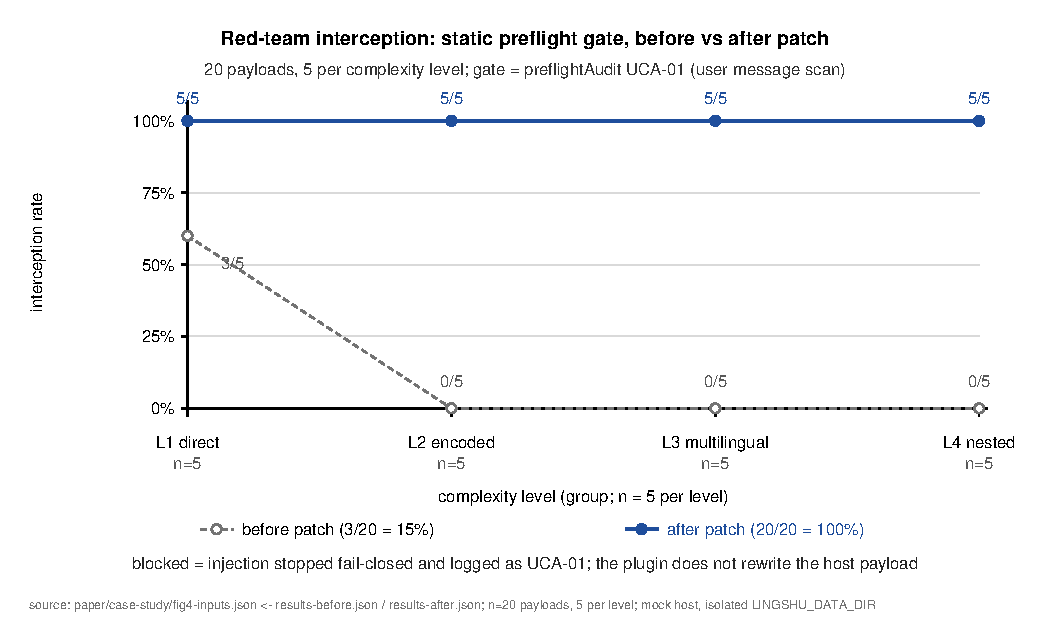
\includegraphics[width=0.98\columnwidth]{figures/fig4-redteam.pdf}
\caption{Case-study patch loop. Interception of twenty mutated payloads before and
after a static rule-layer patch, by construction complexity (L1 direct, L2
encoded, L3 multilingual, L4 nested; $n=5$ per level). Before: 3/20 (15.0\%);
after: 20/20 (100\%). Source:
\texttt{paper/\allowbreak{}case-\allowbreak{}study/\allowbreak{}results-\allowbreak{}before.\allowbreak{}json} and \texttt{results-\allowbreak{}after.\allowbreak{}json};
figure inputs \texttt{paper/\allowbreak{}case-\allowbreak{}study/\allowbreak{}fig4-\allowbreak{}inputs.\allowbreak{}json}.}
\label{fig:redteam}
\end{figure}

\paragraph{What this does and does not show.} It shows that the rule layer is
\emph{operationally patchable}: a single static normalisation pass plus vocabulary
extension moves the same twenty mutations from 15\% to 100\% interception without
touching the product architecture, and each interception is attributable. It does
not show generalisation. The twenty payloads are the patch set, so 100\% is an
in-sample number; the held-out paraphrases remain at 0/20 in each corpus (0/40 in
total; the engine-side gate is unchanged by this plugin-side patch), and the
false-positive cost of wider vocabularies is not measured here. The
\texttt{blocked} state also means only that injection was stopped and recorded:
the host still delivers the user message, so the model may read the attack text.
We therefore treat this as a case study of the patch loop---the evidence that
motivates automated adversarial co-evolution as future work
(Section~\ref{sec:conclusion})---and not as a claim of semantic defence.

\section{Discussion}\label{sec:discussion}

\paragraph{Why a control plane rather than a better memory.} Under I1, a
sharper memory is also a sharper hazard: the more faithful a retrieved statement
is, the more tempting it becomes to present it as current fact. Moving the
design effort from retrieval quality to admission and degradation addresses the
failure surface directly, at the cost of leaving retrieval quality roughly where
it was.

\paragraph{Tension 1: a fail-open majority with a single fail-closed locus.}
The asymmetry is deliberate---a safety failure must block, a functional failure
must stay usable---but it has a price: functional failures can be silent. The
compensation is observability rather than symmetry. Every dropped block carries
a reason code, downgrades are recorded rather than raised, and each turn emits
an event that can be replayed offline. This does not make silent failure
impossible; it makes it attributable after the fact.

\paragraph{Tension 2: a frozen instrument versus a learning loop.} If the
evaluation instrument is writable, the first thing a learning loop learns is to
edit the exam. Freezing metric definitions, replay set, and guardrail thresholds
prevents that, but shrinks the space in which learning can help. Our own search
illustrates the price: across 972 parameter configurations, no configuration
improved the objective by more than the practical-significance threshold
($\Delta < 5\times10^{-4}$), while all six level-1 retrieval parameters became
identifiable. We report it as a methodological result about the instrument, not
about performance.

\paragraph{Tension 3: self-contained plugin versus a single source of truth.} A
host plugin must be installable without a Python runtime, so the control
parameters exist in three places: the authoritative rules file, the host patch
configuration, and the plugin defaults. A 66-key comparison detects drift, but
detecting drift is not proving behavioural equivalence. The honest description
of the port is a re-implementation with a documented divergence list, not a
binding.

\paragraph{Costs.} Four costs are visible in the current artefacts. First,
budget: injected blocks compete with conversation history, and the trade is
governed by static weights that are themselves guesses. Second, latency: the
control plane is designed to stay within a small self-imposed budget, but that
budget is a target, not a measurement. Third, maintenance: two implementations
of the same semantics must be kept aligned by hand. Fourth, audit volume: 308
audit events over eight real turns is a nontrivial storage and inspection load.

\paragraph{Transferability.} Two layers should be separated. The mechanism layer
---threshold semantics, failure semantics, the frozen-instrument discipline---is
host-agnostic and can be specified independently of any API. The wiring layer
---section-based prompt injection, hook names, the approval seam---is specific
to one host. Porting therefore requires re-deriving the wiring and re-checking
each documented divergence against the new host.

\paragraph{Reachability versus effect size.} The evidence in this paper
establishes three things: the mechanisms are reachable in a real host, the
contract executes, and failures are auditable and replayable. It does not
establish a significant positive effect size on large-scale real traffic. That
gap is structural rather than an oversight: measuring such an effect requires
traffic we cannot manufacture and interventions we should not run on someone
else's deployment. It is precisely why the artefacts are open---the engine, the
replay set, the chaos corpora, the pre-registered protocols and the analysis
tools---so that the measurement can be reproduced or refuted by readers with
better access. We would rather publish the instrument and the measured zeros
than a number we cannot defend.

\paragraph{Methodological lesson.} Treating ``what we cannot claim'' as a
first-class artefact turned out to be cheap and repeatedly useful: an
assumptions ledger, a provenance tag on every number, and a frozen instrument
made overclaiming a mechanical rather than a rhetorical failure. We recommend
the practice independently of this system.

% ============================================================================
% 08-limitations.tex - Limitations (target 450--550 words)
% The four frozen research directions appear ONLY here (paper rule).
% Framing-only terms (VSM, rate-distortion) may appear here as explicit
% non-implementations; they must not appear as implemented mechanisms.
% ============================================================================

\section{Limitations}\label{sec:limitations}

\paragraph{Evidence scale, stated once.} Five limits bound every claim here, and
we state them once rather than scattering them. (i)~\emph{Parameters}: all have
provenance \texttt{guess}; the count of \texttt{measured} parameters is zero. The
phase-shift ratios ($0.70$/$0.85$), the trend threshold ($0.02$), the integral
gains, the ACT-R constants and the weight thresholds are design defaults, so no
threshold may be called tuned, validated or optimal. (ii)~\emph{Real traffic}:
eight real turns, five with a ratio observation, all at ratio $\approx 0$; the
calibration protocol's intake---thirty ratio-observed turns, ten boundary
samples, twenty result labels---is unmet. (iii)~\emph{Small samples}: the
external-baseline pilot is five rounds per cell on one host, one model route and
one day; the host pilot is ten cells, one run each; the mechanism supplement uses
twelve probes per class; the patch case study uses twenty payloads; each
held-out corpus has twenty items.
(iv)~\emph{Effect size}: apart from one pre-registered sign test on the ACT-R
class ($12/12$, $p=2.4\times10^{-4}$), no confidence intervals or $p$-values are
reported, and no forgetting, hallucination or end-to-end interception rate is
measured; proxies are labelled as proxies. The claim is reachability, not effect
size. (v)~\emph{Generalisation}: one host, one model route, tokens estimated from
characters; none of this extrapolates to another host, language or tokenizer.

\paragraph{External-baseline and patch-loop scope.} The three-subject comparison
(Section~\ref{sec:exp:baselines}) inherits the small-sample limit above, and its
subjects do not see the same input shape: the no-plugin host receives the raw
four-turn transcript, while the memory systems receive retrieved memories. The
Mem0 arm's out-of-the-box \texttt{add} path is additive, so the superseded value
is retained in the store unless a deletion is issued explicitly; the limits of
the comparison environment are stated separately below. The
interceptions we report for \system{} are \emph{structural} admission decisions:
the gate stops injection and records it, but the host still delivers the user
message, so the model may read the attack text. The pilot also exposed four
product findings that bound its readings: the fact extractor does not recognise
the natural correction phrasing (F-A) and stores the final question as a fact
(F-B); the tool gateway counts schema errors as blocks and injects hints into
later turns (F-C); and the first model request of a turn uses the previous
turn's injection snapshot, so a one-turn-stale memory can still reach the model
(F-D). The last one makes the S1 model-level answers non-interpretable and they
are marked n/i; the ledger-level supersession and a warm diagnostic are reported
separately. The red-team case study (Section~\ref{sec:exp:case-redteam}) is
in-sample by construction---the twenty payloads are the patch set---and the forty
held-out paraphrases stay at 0/40 because the patch is plugin-side while the
held-out evaluation is engine-side. The patch is a laboratory fork, not a product
change; its false-positive cost on benign traffic is not measured; and the
product architecture, including the absence of any adaptation module, is
unchanged.

\paragraph{Synthetic data and mock assertions.} The replay set is entirely
synthetic and permits a synthetic share of one, which disqualifies it for
deployment decisions. Plugin evidence is mock-host assertions
($188 + 148 + 45 + 15 = 396$) plus the ten-cell pilot above, not sustained
traffic. The trigger vocabularies are dominated by two languages, and token usage
is estimated from characters rather than produced by a tokenizer.

\paragraph{Chaos injection scope.} The chaos faults are synthetic single-shot
injections ($n=1$ per fault), not a sample of production failures. The
never-answering case is cut by an outer 150\,s window rather than a measured
client timeout; the warm state is pre-seeded; the context window is a laboratory
override (\texttt{LINGSHU\_CONTEXT\_WINDOW}) with anchors at section positions
rather than the absolute request head and tail; and one campaign used three
headless calls but fifteen provider requests because the agent loop expands a
call into several steps. Raw transcripts and per-field evidence files are kept,
and every claim in Section~\ref{sec:exp:chaos} is tied to a field rather than to a
summary sentence.

\paragraph{External-baseline environment limits.} The official \texttt{mem0ai}
2.2.1 library was run with a local non-neural hashed-bigram embedder (no
embedding API was available), and its default configuration produced empty
recall on cross-lingual queries. These are limits of our comparison environment,
not claims about Mem0.

\paragraph{Ablation power.} The pre-registered three-arm ablation has been
executed (zero-model, deterministic). Its original design supports only coarse
conclusions: the baseline--system retention difference is definitional, and
twelve probes detect only differences of about 0.5 or larger. A supplement
expands the ACT-R probes to twelve (Section~\ref{sec:exp:mech}), where the effect
becomes significant (12/12, $p=2.4\times10^{-4}$), while two mechanism arms
remain inseparable from the gate by construction. The gate itself points the
other way: zero of the forty held-out paraphrases (two corpora of twenty) are
intercepted (0/40, Section~\ref{sec:exp:heldout}), so lexical coverage is a
boundary, not a defence; the patch case study raises in-sample interception to
20/20 without moving this number.

\paragraph{Implementation debt.} Several mechanisms are implemented and unit
tested but not wired: impasse-driven subgoaling has no caller; the reduction path
has no conflict detector, so its trigger is always \texttt{none}; UCA-03 is
unreachable (refusal is never set); dynamic-weight eviction is never exercised
(the replay budget is never exceeded); the saturation-to-gate link is
caller-supplied. The assembled prompt contains no user text, so user-turn
jailbreaks cannot be caught engine-side; ACT-R implements base-level activation
only.

\paragraph{Interpretive framings are not implementations.} Two academic lenses
appear as \emph{framing-only}: the Viable System Model and a rate-distortion
analogy. Neither has a code locus, parameter or dependency: VSM does not occur in
the implementation and no rate--distortion functional is computed. They position
the work but cannot be cited as evidence.

\paragraph{Frozen research directions.} Four directions are explicitly
\emph{frozen}, \emph{not implemented}, and carry \emph{no engineering evidence}:
(i) action closure (closed-loop tool invocation with side-effect rollback);
(ii) adaptive evolution (meta-learning that rewrites its own search targets);
(iii) collective mind (a multi-agent blackboard); and (iv) multimodal
perception. No prototype, dependency or configuration switch exists
for any of them. Their absence bounds our claims: the control plane
governs prompt assembly, not tool execution, cross-agent coordination or
non-textual input.

\paragraph{Safety scope.} The fail-closed guarantee is behavioural and covers
injection only. We implement no independent crisis-safety pre-layer;
refusal depends on the host safety layer and a prompt-level constitution. We
therefore make no end-to-end safety claim: the structural comparisons of
Section~\ref{sec:exp:baselines} measure admission decisions (gate verdicts and
audit events) plus a small model-side pilot, not a safety rate that would
transfer to other hosts, models or attack distributions.

\section{Conclusion}\label{sec:conclusion}

We described \system{}, a cognition layer that treats prompt assembly as a
control surface. The contribution is the shape of the artefact rather than a new
mechanism: a contract that executes and fails loudly (892 Python assertions
across 14 files, 396 plugin-side assertions), failure semantics in which exactly
one component is fail-closed, and an evaluation discipline in which every
parameter's provenance is explicit and the instrument is frozen. The mechanisms
themselves are adapted from established work---ACT-R base-level activation, STPA
unsafe control actions, Ashby's requisite variety, PID-style anti-windup---and
we present them as adaptations, not inventions.

The evidence we present is structural rather than statistical. The contract
executes and fails loudly; exactly one node can stop a turn, and every block it
issues is attributable to a named unsafe control action; downgrades are recorded
rather than silent. Where a structural comparison is possible, the control plane
changes the outcome at the assembly boundary: a superseded fact is suppressed
instead of accumulating, and a static rule patch lifts interception of twenty
mutated payloads from 3/20 to 20/20. The same instrument also bounds the claim:
held-out paraphrases stay at 0/40, so the gate is a lexical and structural
control, not a semantic guarantee. Establishing effect sizes at traffic scale is
the next measurement; the frozen instrument and the open replay harness exist to
make that measurement possible, not to substitute for it.

\paragraph{Future work.} The case study makes the missing piece concrete: the
patch loop above was written by hand, and its 100\% is in-sample. The natural next
step is \emph{automated adversarial co-evolution}---a laboratory loop in which a
red team proposes mutations and the rule layer proposes patches, with the held-out
set and the benign control as the only acceptance gates. We deliberately keep
this out of the product architecture: the shipped control plane remains a static
VSM/STPA surface, and any co-evolution machinery must live in the evaluation
laboratory, with frozen instruments and a human review step. Closing that loop,
and measuring its false-positive cost, is the core direction of future work.


\appendix
% ============================================================================
% 10-appendix.tex - Appendix: UCA table, parameter/provenance table, reproduction
% This file starts with \appendix, so it is safe whether or not main.tex
% already calls \appendix; it must be \input last.
% Requires: booktabs (tables are tabular-only, no multirow dependency).
% ============================================================================

\appendix

\section{Safety control actions (UCA-01--08)}\label{sec:app:uca}

Table~\ref{tab:uca} reproduces the eight unsafe control actions of the
gate as defined in the implementation (the source strings are Chinese and are
translated here). The table, the two trigger word lists and the verdict logic are
hardcoded at
\texttt{engine/control.py:175--188} and \texttt{engine/control.py:191--232};
checks are evaluated in code order, and any hit among UCA-01--07 sets the
verdict to \texttt{block}. UCA-08 is downgrade-only: it is recorded in the
\texttt{downgrades} field and never changes the verdict.

\begin{table}[t]
\centering\small
\caption{Unsafe control actions and their responses. ``Marker'' is a fixed
five-character anchor sentinel beginning with U+3016; ``fact block'' is the
rendered fact block \texttt{f}.}\label{tab:uca}
\begin{tabular}{@{}p{0.08\textwidth}p{0.42\textwidth}p{0.34\textwidth}p{0.09\textwidth}@{}}
\toprule
ID & Definition (translated from the code table) & Detection condition & Response \\
\midrule
UCA-01 & Injected content overrides constitutional constraints & any override phrase in $p$ (\texttt{:207--208}) & block \\
UCA-02 & Constitution verification failed but injection continues & $\neg\mathrm{frozen\_ok}$ (\texttt{:209--210}) & block \\
UCA-03 & Style/emotion injected in a refusal scene & $\mathrm{refuse} \land \mathrm{style\_injected}$ (\texttt{:211--212}) & block \\
UCA-04 & Memory content asserted as current fact (unsourced) & any unsourced phrase in $f$ (\texttt{:213--214}) & block \\
UCA-05 & Budget truncation evicts the constitution & $\neg\mathrm{constitution\_injected}$ (\texttt{:215--216}) & block \\
UCA-06 & Unresolved conflict not reduced & unresolved $\land \neg$fallback (\texttt{:217--218}) & block \\
UCA-07 & Persona anchor missing during a phase shift & prefeed $\land$ marker $\not\subseteq p$ (\texttt{:219--220}) & block \\
UCA-08 & Integration continues after saturation & $\exists k: s_k$ (\texttt{:221--223}) & downgrade only \\
\bottomrule
\end{tabular}
\end{table}

\section{Parameters and provenance}\label{sec:app:params}

Table~\ref{tab:params} lists every numeric parameter touched by the mechanisms
in Section~\ref{sec:method}. The authoritative source is
\texttt{rules/decay-params.yaml}; \texttt{engine/config.py} is a zero-dependency
shadow copy, cross-checked key by key by \texttt{tools/check\_config\_sync.py}
(66 keys, 0 failures). \textbf{All entries are \texttt{provenance: guess}}; the
number of measured parameters is zero
(\texttt{acceptance/provenance-candidates.json} reports
\texttt{upgrade\_eligible: false} for every entry).

\begin{table}[t]
\centering\footnotesize
\caption{Numeric parameters, authoritative rule-file line, value, provenance and
code shadow. ``guess'' is a design default, not a calibrated value.}\label{tab:params}
\begin{tabular}{@{}p{0.25\textwidth}p{0.42\textwidth}p{0.18\textwidth}p{0.11\textwidth}@{}}
\toprule
Parameter key & Value & Provenance & Shadow \\
\midrule
\texttt{actr.d}, \texttt{actr.ref}, \texttt{actr.lo}, \texttt{actr.hi} & 0.5, 0.001 d, $-3.0$, $1.0$ (\texttt{:217--221}) & guess & \texttt{config.py:90--95} \\
\texttt{memory.actrWeight} & 0.6 (\texttt{:18}) & guess\textsuperscript{a} & \texttt{config.py:21} \\
\texttt{memory.decay.tau.*} & 7, 30, 90 d (\texttt{:39--48}) & guess & \texttt{config.py:15--19} \\
\texttt{control.integralKi} / \texttt{Cap} / \texttt{Leak} / \texttt{Deadband} & 0.15 / 0.4 / 0.05 / 0.02 (\texttt{:224--233}) & guess & \texttt{config.py:97--100} \\
\texttt{control.phaseShiftRatio} / \texttt{HardRatio} & 0.70 / 0.85 (\texttt{:228--233}) & guess & \texttt{config.py:101--102} \\
\texttt{control.trendThreshold} / \texttt{ratioMax} / \texttt{historyCapacity} & 0.02 / 1.5 / 64 (\texttt{:230--233}) & guess & \texttt{config.py:104--106} \\
\texttt{compose.weights.fact} / \texttt{organization} / \texttt{style} / \texttt{retrieval} & 0.70 / 0.50 / 0.40 / 0.45 (\texttt{:239--247}) & guess & \texttt{config.py:50--53} \\
\texttt{compose.weights.boost*} & 0.50 / 0.35 / 0.40 (\texttt{:243--247}) & guess & \texttt{config.py:54--56} \\
\texttt{compose.weights.styleBoostThreshold} & 0.6 (\texttt{:246}) & guess & \texttt{config.py:58} \\
\texttt{memory.retrieval.topK} & 3 (\texttt{:20}) & guess & \texttt{config.py:22} \\
\texttt{memory.recallBudget.tokenBudgetDefault} / \texttt{maxReturned} & 900 / 3 (\texttt{:70--71}) & guess\textsuperscript{a} & \texttt{config.py:25} \\
\texttt{memory.potency.archiveThreshold} & 0.15 (\texttt{:50}) & guess\textsuperscript{a} & \texttt{config.py:20} \\
\texttt{compose.injectionTokenRatioMax} & 0.15 (\texttt{:236}) & none\textsuperscript{b} & \texttt{config.py:45} (\texttt{tokenRatioMax}) \\
\texttt{metacog.emotionCapIntensity} & 0.6 & no rule key\textsuperscript{c} & \texttt{config.py:30} \\
\texttt{ASSUMED\_CONTEXT\_TOKENS} & 8000 & no rule key\textsuperscript{c} & \texttt{compose.py:36} \\
\bottomrule
\end{tabular}
\end{table}

\noindent\textsuperscript{a}~The block carries no inline provenance key; the
file header states that all values are guesses (\texttt{:4}), and the enclosing
section repeats \texttt{provenance: guess}.
\textsuperscript{b}~The rule key exists but is not compared by the
consistency tool (key-name mismatch against the shadow).
\textsuperscript{c}~Hardcoded in code; documented as a single-source exception.
These three exceptions are the only places where a numeric value does not flow
from a checked rule-file key.

\section{Reproduction commands and assertion inventory}\label{sec:app:repro}

All Python commands below were executed on the reference implementation while
preparing this paper. The environment variable is required on Windows because
one assertion name contains U+2212, which the default console code page cannot
encode; without it the run aborts on printing, not on an assertion failure.

\begin{verbatim}
$env:PYTHONIOENCODING = "utf-8"
python tests/test_control.py                  # 161 passed, 0 failed
python tests/test_pipeline_integration.py     #  65 passed, 0 failed
python tests/test_constitution.py             #  26 passed, 0 failed
python tools/check_config_sync.py             #  66 ok, 0 fail, 0 skipped
python tools/gen_impl_status.py --check       #  OK (status matrix current)
python tools/run_learning.py --json           #  recall_at_3 = 1.0
node plugin/dsh-lingshu/host-sim.mjs --assert #  documented 188 assertions
node plugin/dsh-lingshu/control-sim.mjs --assert # documented 148 assertions
node plugin/dsh-lingshu/stress.mjs --assert   #  documented 45 assertions
\end{verbatim}

Table~\ref{tab:assertions} attributes the executed Python assertions to the
mechanisms of Section~\ref{sec:method}. Counts are executions, not call sites:
one call site inside a loop runs once per iteration (e.g.\ the top-$k$ slot
check). Plugin assertion counts are those recorded by the project and were not
re-executed for this paper.

\begin{table}[t]
\centering\footnotesize
\caption{Assertion inventory. ``Run'' is the number of assertion executions
observed; ``site'' is the test-file line where the test function starts.}\label{tab:assertions}
\begin{tabular}{@{}p{0.36\textwidth}p{0.34\textwidth}p{0.10\textwidth}p{0.12\textwidth}@{}}
\toprule
Mechanism & Test function (file) & Run & Site \\
\midrule
ACT-R base level & \texttt{test\_actr\_activation} (\texttt{test\_control.py}) & 15 & \texttt{:58} \\
ACT-R dual channel & \texttt{test\_actr\_dual\_channel} (\texttt{test\_control.py}) & 7 & \texttt{:103} \\
Top-$k$ slot contract & \texttt{test\_topk\_slot\_contract} (\texttt{test\_control.py}) & 9 & \texttt{:143} \\
Integral feedback & \texttt{test\_integral\_baseline} (\texttt{test\_control.py}) & 18 & \texttt{:177} \\
Phase-shift monitor & \texttt{test\_phase\_shift\_monitor} (\texttt{test\_control.py}) & 22 & \texttt{:258} \\
Requisite-variety guard & \texttt{test\_requisite\_variety\_guard} (\texttt{test\_control.py}) & 11 & \texttt{:342} \\
Pre-flight gate & \texttt{test\_preflight\_audit} (\texttt{test\_control.py}) & 33 & \texttt{:387} \\
Dynamic weights & \texttt{test\_compose\_weights} (\texttt{test\_control.py}) & 29 & \texttt{:484} \\
Single-source parameters & \texttt{test\_params\_single\_source} (\texttt{test\_control.py}) & 8 & \texttt{:623} \\
Impasse & \texttt{test\_impasse} (\texttt{test\_control.py}) & 7 & \texttt{:668} \\
Pipeline integration & nine functions & 65 & \texttt{test\_pipeline\_integration.py:46--284} \\
Constitution audit & five functions & 26 & \texttt{test\_constitution.py} \\
\bottomrule
\end{tabular}
\end{table}

The gate-level measurements quoted in the text were produced with the same
token-free call used by the chaos executor
(\texttt{tools/run\_chaos.py:443--446}): the sample text is passed as the
\texttt{prompt} argument with \texttt{frozen\_ok=True} and
\texttt{constitution\_injected=True}, which isolates UCA-01. This is a unit-level
coverage check on the gate's scan surface, not an end-to-end interception
measurement.

\subsection{Test Rigor and Anti-Cheating Audit}\label{app:audit}

This appendix records how the test evidence quoted in
Section~\ref{sec:engineering} was produced. All numbers below come from one
audit bundle dated 2026-10-27: two reviewer reports (mutation testing; assertion
strength and coverage), one consolidated rigor report, and two machine-readable
result files, all archived under \texttt{acceptance/audit/}. Nothing here is
reconstructed from memory: every figure is a field of the archived JSON or a
table of the reports.

\begin{table*}[t]
\centering
\caption{Mutation matrix. A mutant counts as killed only when an assertion
fails; crash-only kills are excluded (0 observed). The two surviving mutants
after supplementation are equivalent mutants, not test weaknesses. The rules
file mutants are caught by cross-file consistency assertions rather than by
behavioural ones.}
\label{tab:mutants}
\small
\begin{tabular}{lrrrrl}
\toprule
Region & Mutants & Killed & Rate & Survivors & After supplement \\
\midrule
\texttt{plugin/control.js}      & 16 & 15 & 93.8\% & 1 equivalent      & 15/15 non-equivalent \\
\texttt{plugin/\allowbreak{}memorywriter.\allowbreak{}js} &  5 &  3 & 60.0\% & 2 real blind spots & 5/5 \\
\texttt{plugin/index.js}        &  8 &  6 & 75.0\% & 2 real blind spots & 8/8 \\
\texttt{engine/control.py}      & 11 & 10 & 90.9\% & 1 equivalent      & 10/10 non-equivalent \\
\texttt{rules/\allowbreak{}decay-\allowbreak{}params.\allowbreak{}yaml}&  4 &  4 & 100\%  & 0                 & 4/4 \\
\midrule
Total                           & 44 & 38 & 86.4\% & 4 real + 2 equiv. & 42/44 (95.5\%); 42/42 non-equivalent \\
\bottomrule
\end{tabular}
\end{table*}

\begin{table*}[t]
\centering
\caption{Coverage and exception paths. Panel (a): Python line and branch
coverage by group, measured with a PEP~669 \texttt{sys.monitoring} tracer.
Panel (b): JavaScript coverage measured from V8 data; the block column is an
approximation of branch coverage, not true branch coverage. Panel (c):
assertion-strength grading and the strict exception-path share. Coverage is
reported as measured, and is not used to claim the absence of dead code.}
\label{tab:coverage}
\small
\textbf{(a) Python coverage}\\[2pt]
\begin{tabular}{lrrrrrrr}
\toprule
Group & Files run & Exec.\ lines & Covered & Line \% & Branches & Covered & Branch \% \\
\midrule
\texttt{engine/}        & 20/20 & 2{,}319 & 2{,}086 & 89.95 & 648  & 523  & 80.71 \\
\texttt{tools/}         & 3/26  & 8{,}023 & 2{,}641 & 32.92 & 1{,}794 & 527 & 29.38 \\
\texttt{integrations/}  & 1/1   &    99 &    56 & 56.57 & 18   & 12   & 66.67 \\
Total                   & 47    & 10{,}441 & 4{,}783 & 45.81 & 2{,}460 & 1{,}062 & 43.17 \\
\bottomrule
\end{tabular}\\[6pt]
\textbf{(b) JavaScript coverage (block column is approximate)}\\[2pt]
\begin{tabular}{lrrrr}
\toprule
File & Exec.\ lines & Covered & Line \% & Block/branch \% \\
\midrule
\texttt{control.js}      &   360 &   341 & 94.72 & 74.81 \\
\texttt{goalrelation.js} &   181 &   163 & 90.06 & 71.53 \\
\texttt{index.js}        & 1{,}066 & 1{,}018 & 95.50 & 64.00 \\
\texttt{memorywriter.js} &   182 &   179 & 98.35 & 56.19 \\
Total                    & 1{,}789 & 1{,}701 & 95.08 & 66.22 \\
\bottomrule
\end{tabular}\\[6pt]
\textbf{(c) Assertion strength and exception paths}\\[2pt]
\begin{tabular}{@{}l r r r p{0.28\textwidth}@{}}
\toprule
Quantity & Python & JavaScript & Sample & Note \\
\midrule
Sampled assertions            & 165 &  73 & 238 & fixed seed; tautologies = 0 \\
Strong / weak (sample)        & 125 / 40 & 54 / 19 & 238 & 179 strong (75.2\%), 59 weak \\
Full heuristic scan           & 597 / 227 / 1 & 278 / 89 / 0 & 1{,}192 & strong/weak/tautology; 26.6\% weak-or-tautological \\
Strict exception share        & 199/825 = 24.1\% & 82/367 = 22.3\% & -- & relaxed upper bounds 43.3\% / 54.2\% \\
\bottomrule
\end{tabular}
\end{table*}

\paragraph{What the tables do not show.} Three caveats belong next to the
numbers. First, \texttt{engine/control.py} has no unexecuted line under the
tested configuration ($141/141$ lines, $56/56$ branches), but this does not
establish the absence of dead code: two equivalent mutants survive precisely
because a branch is unreachable, and unreachability is what a coverage number
cannot distinguish from an untested branch. Second, the whole-repository Python
figure of $45.81\%$ is pulled down by \texttt{tools/} ($32.92\%$; 3 of 26 files
executed), and \texttt{tools/} coverage is itself a lower bound because
subprocess-invoked tools are recorded as unexecuted. Third, the repository has
no version-control history, so the audit can certify the current state but
cannot certify that no assertion was weakened at an earlier time.

\paragraph{Reproduction.} The bundled files are
\texttt{acceptance/\allowbreak{}audit/\allowbreak{}mutation-\allowbreak{}results-\allowbreak{}2026-\allowbreak{}10-\allowbreak{}27.\allowbreak{}json} (per-mutant outcomes,
survivor analysis, and the before/after SHA-256 lists) and
\texttt{acceptance/\allowbreak{}audit/\allowbreak{}coverage-\allowbreak{}summary-\allowbreak{}2026-\allowbreak{}10-\allowbreak{}27.\allowbreak{}json} (per-file line and
branch data), with the human-readable reports alongside them. Full suites:
fourteen Python test files (892 assertions) and four JavaScript suites (396
assertions). Mutation replay uses a full copy of the repository; the mutation
driver, per-round raw output, and the independent re-run log are archived in the
audit bundle and available from the authors, since they sit outside the
repository so that no reviewer-run artefact can alter the submitted tree. On
Windows, three Python test files require a temporary-directory shim because the
sandbox blocks \texttt{tempfile.\allowbreak{}mkdtemp()}; the shim replaces temporary-directory
creation only and changes no assertion and no line of implementation code.

% =====================================================================
% 10c-appendix-tool.tex -- T-UCA full table, fields, reproduction
% SOURCE OF TRUTH: docs/24 (tool-gateway UCA contract, v1.1: T-UCA-01..16,
% policy_version "t-uca-1.1"; audit field for tool-side ids is `ucas`).
% PENDING NUMBERS (fill only from a5 real outputs): N/M/K/A/X in 06e.
% =====================================================================

\subsection{Tool-Call Unsafe Control Actions ({T-UCA})}\label{app:tuca}

This appendix mirrors the tool-side matrix that the implementation encodes. The
matrix is defined once, in the project's tool-gateway contract
(\texttt{docs/24}), and is implemented twice---as \texttt{engine/\allowbreak{}tool\_\allowbreak{}gateway.\allowbreak{}py}
(pure functions, zero dependencies) and as
\texttt{plugin/\allowbreak{}dsh-\allowbreak{}lingshu/\allowbreak{}tool-\allowbreak{}gateway.\allowbreak{}js} (same semantics)---with both rule
tables machine-synchronised from the contract's rule array, so that each
identifier, verdict and hint text agrees row by row. The namespace is disjoint
from the injection-side UCA-01--08; the two are related only by ordering:
injection pre-flight runs before the model call, the tool gate runs after a call
is emitted and before execution. The contract's policy version is
\texttt{t-uca-1.1} (the \texttt{v1.0.0-paper-baseline} snapshot, commit
\texttt{d551079}, 2026-10-27), and the field carrying tool-side identifiers in the audit
event is named \texttt{ucas} (same spelling as the injection-side field, but a
different event type: \texttt{tool\_gate.ucas} may contain only
\texttt{T-UCA-xx}, \texttt{audit.ucas} only \texttt{UCA-0x}).

\begin{table*}[t]
\centering
\caption{Tool-side unsafe control actions (\texttt{docs/24} v1.1, policy
\texttt{t-uca-1.1}, paper baseline). Sixteen rules: thirteen block, three degrade (a degrade
falls back to block when no approval channel exists). No rule returns
\emph{allow}; allow is the default policy for read-only calls that match no rule.
The \emph{group} column follows the contract's grouping and is not a runtime
field.}
\label{tab:tuca}
\scriptsize
\begin{tabular}{llp{3.6cm}lp{2.2cm}l}
\toprule
ID & Group & Trigger (contract summary) & State inputs & Verdict & Test case \\
\midrule
T-UCA-01 & state        & mutating call while variety fallback or unresolved conflict is active & variety, conflict & block & \texttt{test\_tuca\_01} \\
T-UCA-02 & data         & credential or secret material in arguments or target & capabilities & block & \texttt{test\_tuca\_02} \\
T-UCA-03 & mutation     & destructive delete/overwrite without exact matching confirmation & --- & block & \texttt{test\_tuca\_03} \\
T-UCA-04 & mutation     & write to frozen/protected path (incl.\ \texttt{engine/}, \texttt{plugin/} sources) & frozen\_ok & block & \texttt{test\_tuca\_04} \\
T-UCA-05 & network/exec & network egress outside the (default empty) allowlist & capabilities & block & \texttt{test\_tuca\_05} \\
T-UCA-06 & network/exec & arbitrary code execution (capability or execution-shaped args) & capabilities & block & \texttt{test\_tuca\_06} \\
T-UCA-07 & shape        & oversized, deeply nested or multi-encoded payload & --- & block & \texttt{test\_tuca\_07} \\
T-UCA-08 & shape        & unregistered tool or incomplete registry entry & tool\_registry & block & \texttt{test\_tuca\_08} \\
T-UCA-09 & shape        & schema violation, delimiter/control-character injection, homoglyph tool name & tool\_registry & block & \texttt{test\_tuca\_09} \\
T-UCA-10 & state        & mutating call while context phase is critical & phase & degrade$\rightarrow$block & \texttt{test\_tuca\_10} \\
T-UCA-11 & audit        & incomplete audit context (missing session/turn/call id) & audit\_context & block & \texttt{test\_tuca\_11} \\
T-UCA-12 & shape        & capability neither declared nor granted & capabilities & block & \texttt{test\_tuca\_12} \\
T-UCA-13 & state        & saturated affective baseline with irreversible write, unconfirmed & saturated & degrade$\rightarrow$block & \texttt{test\_tuca\_13} \\
T-UCA-14 & mutation     & frozen-region check failed and call is mutating & frozen\_ok & block & \texttt{test\_tuca\_14} \\
T-UCA-15 & mutation     & path escapes the workspace (\texttt{..}, absolute, drive, UNC, null byte) & --- & block & \texttt{test\_tuca\_15} \\
T-UCA-16 & state        & destructive call while context phase is shift & phase & degrade$\rightarrow$block & \texttt{test\_tuca\_16} \\
\bottomrule
\end{tabular}
\end{table*}

\paragraph{Default policy and evaluation order.} Unknown, unregistered or
undecidable calls are blocked (\mbox{fail-closed}); read-only calls that match no rule
are allowed and logged; a mutating call whose phase is unknown is blocked; a
parse failure is blocked with an explicit \texttt{parse\_error} reason rather
than inferred intent. When several rules match, the verdict takes the highest
severity (block over degrade over allow) and \emph{all} matched identifiers are
recorded in \texttt{ucas} without truncation. Evaluation order puts static checks
first, then the state-dependent rules, and the audit rule last:
\texttt{T-\allowbreak{}UCA-\allowbreak{}01, 02, 03, 04, 05, 06, 07, 08, 09, 12, 14, 15, 10, 13, 16, 11}.
A \texttt{degrade} means the original call is not executed: the caller returns a
strong hint, sets \texttt{requires\_\allowbreak{}confirmation}, and requires an explicit human
confirmation through the host approval seam; a degrade with no approval channel
is treated as a block (\texttt{degraded\_to}). The gate never executes a payload
and never rewrites arguments; it classifies, consults state, and returns a
verdict.

\paragraph{State inputs and tool classes.} The gate consumes only state that
already exists in the system: \texttt{variety\_fallback} and
\texttt{unresolvedConflict} (from the conflict and variety machinery),
\texttt{phase} (from the preemptive monitor), \texttt{saturated} (from the
integral baseline), \texttt{frozen\_ok} (from the frozen-region check),
\texttt{capabilities} (declared versus granted), \texttt{audit\_context}, and the
tool registry. Tool classes are closed and static---\texttt{read}, \texttt{write},
\texttt{destructive}, \texttt{exec}, \texttt{network}---with \texttt{write},
\texttt{destructive}, \texttt{exec} and \texttt{network} treated as mutating and
\texttt{read} as read-only; a payload cannot declare its own class. Finer
semantics (for example which arguments name a path) live in the registry's
capability declarations rather than in the class enum.

\paragraph{Audit fields.} Each verdict produces one \texttt{tool\_gate} event:
\texttt{schema}, \texttt{policy\_version}, \texttt{call\_id},
\texttt{session\_id}, \texttt{turn\_id}, \texttt{tool}, \texttt{tool\_class},
\texttt{verdict}, \texttt{allowed}, \texttt{ucas}, \texttt{degraded\_to},
\texttt{requires\_\allowbreak{}confirmation}, \texttt{reason}, a nested
\texttt{audit} block (\texttt{args\_digest}, \texttt{args\_keys},
\texttt{args\_bytes}, \texttt{args\_preview}, \texttt{phase},
\texttt{variety\_fallback}, \texttt{frozen\_ok}, \texttt{saturated}), and a
\texttt{snapshot} of the target (path, modification time, hash) used to check
that the object judged is the object executed. Argument digests and key lists
are recorded instead of raw secret-bearing arguments. In the host plugin the
same event drives a clarification flag that surfaces as a strong hint on the next
turn.

\paragraph{Reproduction.} \texttt{python tests/\allowbreak{}test\_\allowbreak{}tool\_\allowbreak{}gateway.\allowbreak{}py} exercises
dangerous, benign, state-gated and cross-language cases (as run for this draft:
79 passing assertions, 20/20 dangerous blocked, 0/8 benign blocked, 20/20
cross-language agreement);
\texttt{node plugin/\allowbreak{}dsh-\allowbreak{}lingshu/\allowbreak{}tool-\allowbreak{}gateway-\allowbreak{}sim.\allowbreak{}mjs -\allowbreak{}-\allowbreak{}assert} checks the rules
individually in JavaScript (65 checks);
\texttt{python tools/\allowbreak{}run\_\allowbreak{}actuator\_\allowbreak{}demo.\allowbreak{}py} drives the reference loop and emits
the JSON cited in Section~\ref{sec:actuator}. The frozen blind held-out set is
\texttt{paper/\allowbreak{}ablation/\allowbreak{}tool/\allowbreak{}heldout-\allowbreak{}tool-\allowbreak{}calls-\allowbreak{}v1.\allowbreak{}jsonl} (ten calls, two per
family; SHA-256
\texttt{\seqsplit{f68fc1b3f19fc37e43b9856096d29b9a55de7dee9bf664a9b9a9592e070576d4}}); it
is evaluated by a party other than its author, under two regimes (arguments
only, and arguments with context), because the conflict family depends on
context.

\paragraph{Boundaries recorded with the matrix.} The host exposes no
pre-dispatch hook, so plugin-side blocking is limited to tools routed through
\texttt{guardTool}; engine-side pre-blocking is a reference loop, not a product
enforcement point. Tools executed outside the gateway are not gated. The gate is
a static checker, so parsing is its own attack surface, and its false-positive
rate is uncalibrated in the absence of real traffic. The contract also records
known false-positive surfaces (confirmation fatigue for writes during the
critical phase, legitimate maintenance of protected paths, documents that merely
discuss credential formats, and large legitimate imports). These are repeated
here because a matrix in an appendix is exactly where a reader is most likely to
mistake a rule table for an enforcement guarantee.

% ============================================================================
% 10d-appendix-hostpilot.tex -- Host-side pilot details (moved out of the main
% experiments text under the "subtract and amplify" revision).
% Sources: paper/host-validation/REPORT.md and calls.json (single-message pilot);
%          paper/host-validation/s4-long-session/{calls.json, REPORT.md} (S4).
% Table/numbers are unchanged from the main text version; only the location moved.
% ============================================================================

\subsection{Real-host pilot details}\label{app:hostpilotdata}

This appendix holds the two host-side pilots whose headlines remain in
Section~\ref{sec:exp:host} and Section~\ref{sec:exp:s4}. Nothing here is a new
measurement: the numbers are transferred verbatim from the main text and the
archived records, and the two pilots differ in shape (one concatenated request
versus genuine per-turn calls).

\paragraph{Host pilot (single concatenated request).} Ten cells ran on one host,
one model route, one run each: \textsc{Full} (plugin) and \textsc{Baseline} (no
plugin) against three probe phrasings, plus two controls. A cell is one headless
CLI invocation over a 100-turn prompt of 78,565--78,652 bytes---the host-feasible
single-message form (50 flood turns, 49 replay turns, one probe). All 11
invocations, including the feasibility probe, exited zero, with at least 26 model
requests (26--36 estimated, since one CLI invocation is an agent loop) and
193,288 tokens.

The main matrix is a ceiling: 6/6 answers contain the planted codename because
the seed sentence is verbatim in the prompt. Removing that sentence is more
informative: \textsc{Full} reports \texttt{matched=0}, injects no memory section,
and both arms answer not-found---a methodological finding, since compressing a
100-turn dialogue into one 78\,KB message dilutes the query until
query-conditioned retrieval stops hitting. This also questions stress protocols
that concatenate many turns into one prompt. A short-query control isolates the
channel: \textsc{Full} injects the seeded entry and answers the codename, whereas
\textsc{Baseline}, with no memory, takes ten tool steps and answers with the
directory name. That is a mechanism demonstration at $n=1$, not a hallucination
rate. \textsc{Basic} is not applicable on the host: the plugin exposes parameter
defaults but no switch to disable the control layer. In all ten cells the gate
returned \texttt{allow} with an empty UCA list, so the pilot says nothing about
the control layer.

\paragraph{Per-turn long-session pilot (S4).} The last experiment replaces the
single concatenated message with genuine per-turn calls. Two arms---\textsc{Full}
(plugin and control plane) and \textsc{Baseline} (no plugin; the harness prepends
the last $W=3$ turns)---run two 30-turn variants. Settings are planted in turns
1--2, a superseding statement appears at turn 3, and probes at turns 10, 20 and 30
ask for the setting, the superseded value, the interface preference and an
unmentioned cat. Primary delivery is the v1 subset: 60 cells, 60/60 exit zero,
419{,}203 tokens. The full 120-cell run (873{,}198 tokens) is archived and is never
pooled with the primary numbers; the extra variant is a cross-check only.

\begin{table*}[t]
\centering\footnotesize
\caption{Per-turn long-session pilot (S4), primary v1 subset: six probe outcomes
(three probe turns $\times$ two arms), rule-assisted counts. Source:
\texttt{calls.json}, fields \texttt{observations\_\allowbreak{}raw\_\allowbreak{}counts.\allowbreak{}full-\allowbreak{}v1},
\texttt{.baseline-v1}, \texttt{aggregate.*}, \texttt{full\_\allowbreak{}arm\_\allowbreak{}memory\_\allowbreak{}evidence.\allowbreak{}v1},
\texttt{totals\_\allowbreak{}v1\_\allowbreak{}subset\_\allowbreak{}60}; the same record is duplicated in
\texttt{long-\allowbreak{}session-\allowbreak{}2026-\allowbreak{}10-\allowbreak{}27.\allowbreak{}json}.}
\label{tab:s4}
\begin{tabular}{@{}l ccccc@{}}
\toprule
Arm & Setting kept & Stale ALPHA & Unknown ack. & Preference kept & Memory injected \\
\midrule
\textsc{Full} & 0/3 & 0/3 & 3/3 & 1/3 & 3/3 \\
\textsc{Baseline} & 3/3 & 0/3 & 1/3 & 3/3 & 0/3 \\
\bottomrule
\end{tabular}
\end{table*}

Table~\ref{tab:s4} shows the six probe outcomes. Read alone they invite the wrong
conclusion, so two mechanism facts must be read with them. First, \textsc{Full}
did inject memory in all three probe turns, but the content was wrong: the
turn-3 supersession does not match any of the plugin's three supported extraction
patterns (\texttt{plugin/\allowbreak{}dsh-\allowbreak{}lingshu/\allowbreak{}index.\allowbreak{}js:\allowbreak{}1004-\allowbreak{}-\allowbreak{}1011}), so BETA was never
written and the memory's last-wins view has
\texttt{beta\_\allowbreak{}present=false} with the project code still ALPHA---a stale value.
Second, the probe question itself was extracted as a fact: asking for the
interface preference matches the pattern with object ``what'', and that junk
entry superseded the correct preference (one supersede event, in the wrong
direction). \textsc{Full}'s model therefore saw ``code = ALPHA'' and
``preference = what'' and, following invariant~I1 (memory is a reference, never
the current statement), answered that there was no record. That is the designed
behaviour on corrupted input, not a capability ceiling.

\textsc{Baseline}'s apparent retention has a different origin: the window carries
the assistant's own earlier restatements, so BETA and the dark theme survive by
self-repetition rather than through memory, and two answers fabricate turn
references---citing filler turns 7--8 as prior user statements that were in fact
the assistant's own restatements. The pre-registered P-S4a (Full at least as
good as Baseline on setting retention) is therefore \emph{not supported} and is
recorded as \texttt{null}. What this pilot shows is an input-construction defect
interacting with the real boundary of a rule extractor; it cannot be read as
``\textsc{Full} is less capable'' or ``\textsc{Baseline} is better''. With one
chain per arm and variant, one model, one host and rule-assisted counting, we
report counts, not rates. The archived v2 variant repeats the pattern
(\textsc{Full} 0/3, \textsc{Baseline} 2/3) and is not pooled.


\bibliographystyle{plainnat}
\bibliography{refs}

\end{document}
